\documentclass[11pt]{article}
\usepackage[a4paper, total={6.5in, 9.5in}]{geometry}
\usepackage[document]{ragged2e}
\usepackage[bookmarksopen=true,hidelinks]{hyperref}
\usepackage{bookmark}
\usepackage{lipsum}
\usepackage{graphicx}
\usepackage[noadjust]{cite}
\usepackage{float}
\usepackage[numbib]{tocbibind}
\usepackage{multirow}
\usepackage{array}
\usepackage{setspace}
\usepackage{cellspace}
\usepackage{etoolbox}
\usepackage{longtable}
\usepackage[table, svgnames]{xcolor}
\usepackage{titlesec}
\usepackage{amsmath}
\usepackage{pdfpages}
\setcounter{secnumdepth}{4}

\usepackage{fancyhdr}
\fancypagestyle{logo}{
    \fancyhf{} % clears header/footer
    \renewcommand\bottomfraction{0.9}
    \renewcommand\textfraction{0.1}
    \fancyhead[C]{
\includegraphics[ width=\linewidth, keepaspectratio]{./images/header_white.png}}
    \fancyfoot[LE,RO]{\thepage}
}
\pagestyle{logo}


% Glossary
\usepackage[utf8]{inputenc}
\usepackage{glossaries}
\makeglossaries

\newglossaryentry{ARM64}{name=ARM64, description={Advanced RISC Machine, A family of RISC based processors}}
\newglossaryentry{Actix Web}{name=Actix Web, description={A webserver library built ontop of Actix}}
\newglossaryentry{Actix}{name=Actix, description={An implementation of the Actor Model in Rust}}
\newglossaryentry{Actor Model}{name=Actor Model, description={A concurrency managment paradigm that uses message passing between objects rather than locks or atomics}}
\newglossaryentry{Actor}{name=Actor, description={A class that contains message handling callbacks}}
\newglossaryentry{Aptitude}{name=Aptitude, description={A debian package manager that automatically manages updates and installation of software and dependencies}}
\newglossaryentry{Arbiter}{name=Arbitor, description={A thread pool, where each thread is an event loop}}
\newglossaryentry{Babel}{name=Babel, description={A scripting language similar to Javascript with the ability to directly construct HTML snippets}}
\newglossaryentry{Borrow Checker}{name=Borrow Checker, description={A component of the Rust compiler to prevent data races by enforcing data ownership rules.}}
\newglossaryentry{C2C}{name=C2C, description={Cradle to Cradle development to ensure innovating and sustainable products}}
\newglossaryentry{CISC}{name=CISC, description={Complex Instruction Set Computer}}
\newglossaryentry{CSA}{name=CSA, description={Canadian Standards Association is a standards development organization}}
\newglossaryentry{DC}{name=DC, description={Direct current voltage}}
\newglossaryentry{DPU}{name=DPU, description={Data Processing Unit}}
\newglossaryentry{Debian}{name=Debian, description={A Linux based operating system}}
\newglossaryentry{GUI}{name=GUI, description={Graphical User Interface}}
\newglossaryentry{Garbage Collector}{name=Garbage Collector, description={A runtime component of some programming languages that detects and cleans up unused memory.}}
\newglossaryentry{HTTP}{name=HTTP, description={HyperText Transfer Protocol}}
\newglossaryentry{ID}{name=ID, description={Identification}}
\newglossaryentry{IEC}{name=IEC, description={International Electrotechnical Commission}}
\newglossaryentry{IEEE}{name=IEEE, description={Institute of Electrical and Electronics Engineers}}
\newglossaryentry{ISO}{name=ISO, description={the International Organization for Standardization. }}
\newglossaryentry{JQuery}{name=JQuery, description={A Javascript library designed to manipulate HTML}}
\newglossaryentry{MCU}{name=MCU, description={Micro-controller unit}}
\newglossaryentry{MPSC}{name=MPSC, description={Multiple Producer Single Consumer Queue}}
\newglossaryentry{MVC}{name=MVC, description={Model View Controller, a method of orgnanization for GUI implementations}}
\newglossaryentry{PCB}{name=PCB, description={Printed circuit board}}
\newglossaryentry{PoC}{name=PoC, description={Proof of concept is the sample product assembled to explore project feasibility}}
\newglossaryentry{RF}{name=RF, description={Radio Frequency}}
\newglossaryentry{RISC}{name=RISC, description={Reduced Instruction Set Computer}}
\newglossaryentry{RSSI}{name=RSSI, description={Received Signal Strength Indicator}}
\newglossaryentry{React}{name=React, description={A Javascript framework to dynamically generate HTML}}
\newglossaryentry{Rolling Release}{name=Rolling Release, description={Frequent updates of software, without versions}}
\newglossaryentry{Rust}{name=Rust, description={A systems language that focuses on reliability and performance}}
\newglossaryentry{Server Side Rendering}{name=Server Side Rendering, description={Creating HTML files on the server, which can then be directly consumed by the browser without modification to render a GUI}}
\newglossaryentry{ToF}{name=ToF, description={Time-of-Flight is a method for measuring the distance between a sensor and an object}}
\newglossaryentry{UI}{name=UI, description={User Interface}}
\newglossaryentry{UWB}{name=UWB, description={Ultra wide band}}
\newglossaryentry{iOS}{name=iOS, description={Operating system released by Apple Inc.}}
\newglossaryentry{x86-64}{name=x86-64, description={Intel designed CISC family of processors}}


% compile __Requirements_Specification.tex
% run
%makeindex -s __Requirements_Specification.ist -o __Requirements_Specification.gls __Requirements_Specification.glo
% recompile __Requirements_Specification.tex



\begin{document}

%\setboolean{@twoside}{false}
%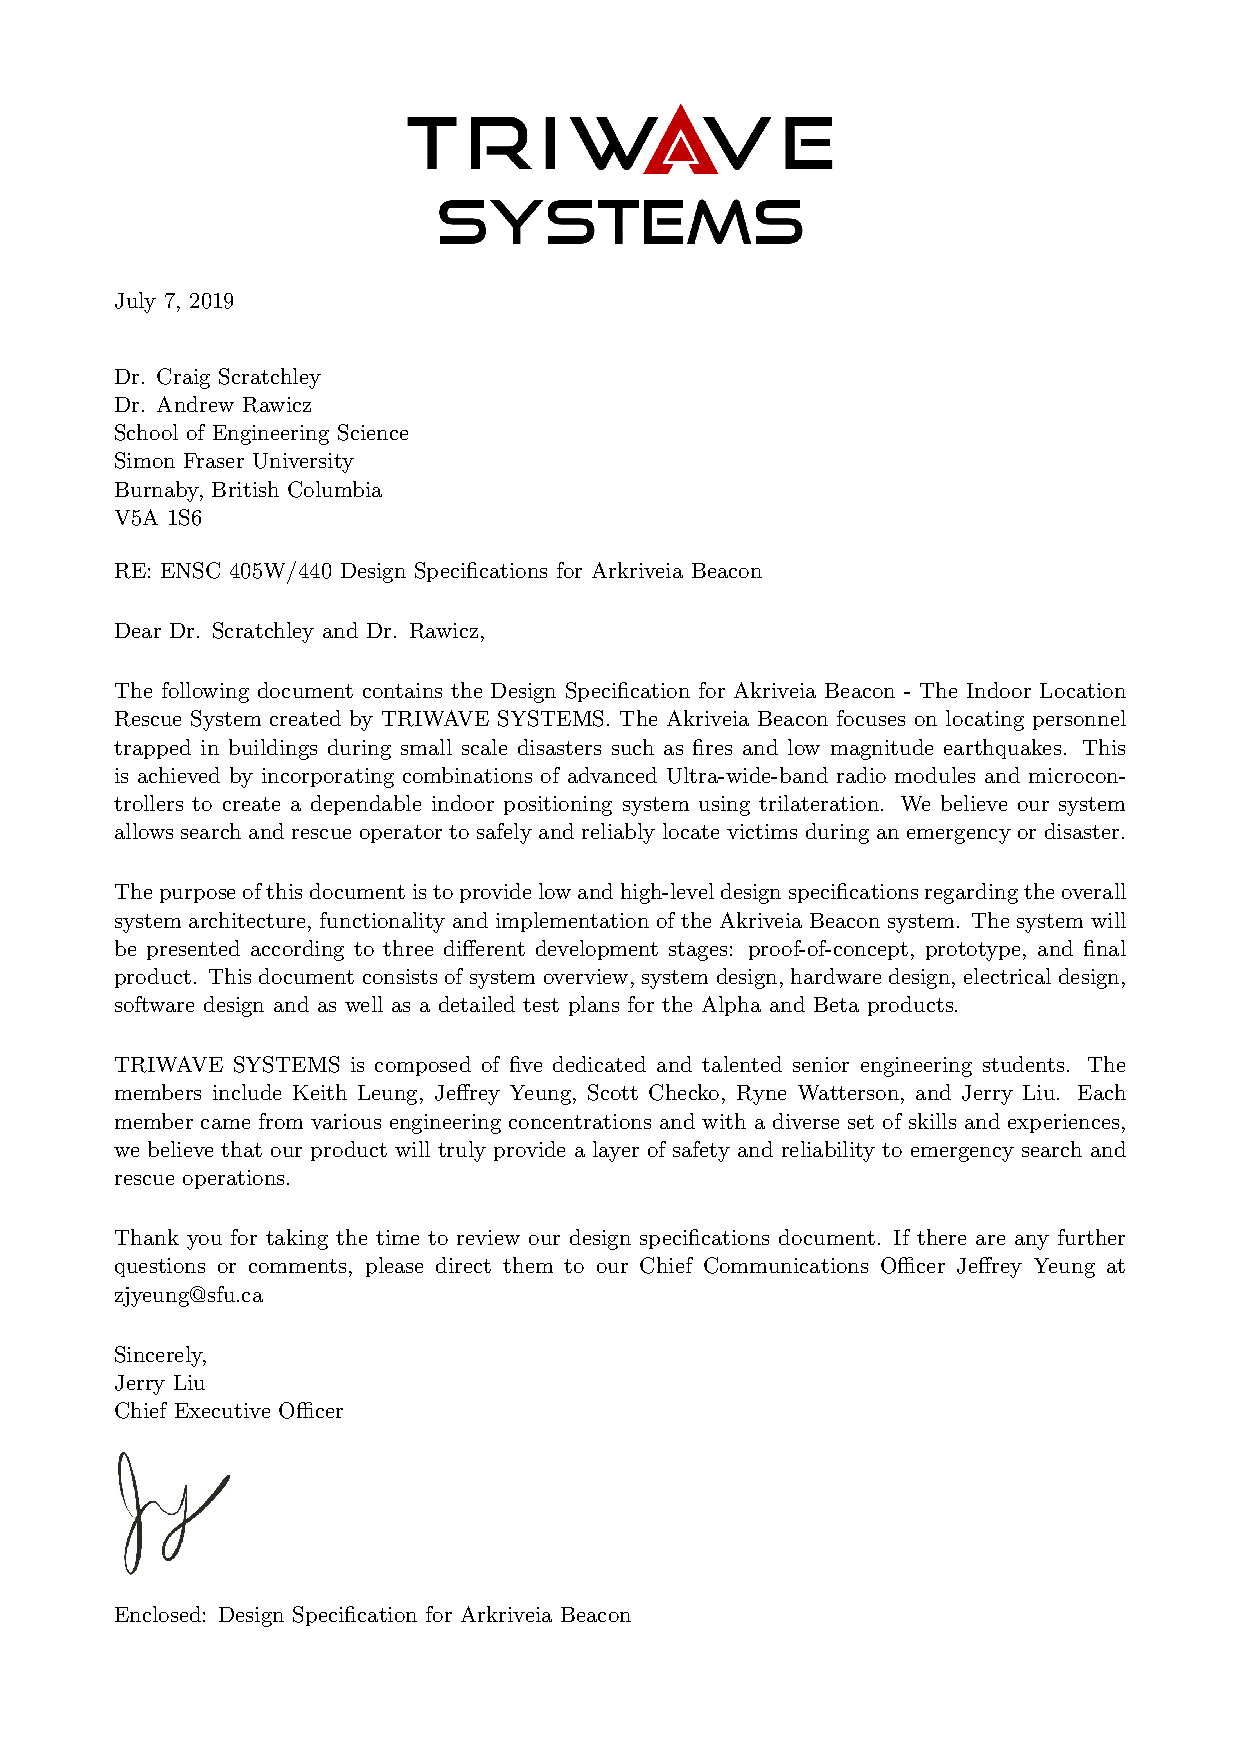
\includepdf[pages={1}]{./images/_Letter_of_transmittal.pdf}
%\setboolean{@twoside}{false}
%
\includepdf[pages={1}]{./images/title_page_white.pdf}

%\documentclass[11pt]{article}
%\usepackage[document]{ragged2e}
%\usepackage[a4paper, total={6in, 9in}]{geometry}
%\usepackage{graphicx}
%\usepackage{float}
%\usepackage{multirow}
%\usepackage{array}
%\begin{document}


\begin{abstract}
\medskip
The Akriveia Beacon by TRIWAVE SYSTEMS focuses on improving the locating and rescue process of personnels trapped in buildings during or after small scale disasters such as fires and low magnitude earthquakes. This is achieved by incorporating an combination of advanced Ultra-wide-band radio modules, microcontroller units and data processing server to create an dependable indoor positioning system using reliable trilateration techniques. Akriveia Beacon allows search and rescue operations to safely and reliably locate victims during and after an emergency or disaster. By pinpointing the exact location of any victim wearing an ID tag, this allows rescue operators minimizing the search and rescue time; which is crucial during the time period right after a disaster strikes.

\bigskip
This document addresses the functional and nonfunctional requirements for Akriveia Beacon - The Indoor Location Rescue System created by TRIWAVE SYSTEMS. From this document, the reader will be able to gain full understanding to the functions and higher-level system design of the Akriveia Beacon. The specifications details system components, and requirements for each specified domains. Additionally aspects of engineering standards, responsibilities, safety, and sustainability of this project are outlined to provide an overview for practices followed by the engineers at TRIWAVE SYSTEMS.

\bigskip
TRIWAVE SYSTEMS is dedicated to creating a reliable and robust system for disaster search and rescue operations with human safety as the pivotal focus.

\end{abstract}
%\end{document}

\pagebreak
\clearpage
\printglossaries
\pagebreak
\begin{spacing}{0.90}
\tableofcontents
\end{spacing}
\pagebreak
\listoffigures
\pagebreak
\listoftables
\pagebreak


\setcounter{section}{0}
\section{Introduction}
\bigskip

\subsection{Background}
Over the last couple of decades urban centers around the world have faced substantial population growth. As a result, the number of large and complex structures in dense urban areas around the world is rapidly increasing. In Canada alone there are approximating 500,000 commercial buildings \cite{R1}. A large population combined with massively complex buildings in relatively dense areas leads to higher risk for damage and casualties in the event of a disaster. Due to increased urbanization and complexity of urban structures, search and rescue operations in indoor urban environments face various complications and uncertainties. According to Statistics Canada, an average of 135 fire related deaths occur with commercial structures each year from 2010 to 2014 \cite{R2}.

\bigskip
In current practices, first responders know little about the situation until arriving on scene. Once responders are on scene, emergency management have to quickly evaluate the situation and take appropriate actions \cite{R3}.  Assessments of the structure are conducted with readily available blueprints of buildings along with limited information of last known location of possible trapped victims, usually derived from witness reports. Situational data are created dynamically during this process and the actual rescue process heavily depends on the situational awareness of the first line of emergency response operators \cite{R4}.

\bigskip
An important issue that must be considered is how emergency first responders should be dispatched inside the building in the event of a disaster in order to minimize search and rescue time. In order to pinpoint locations of trapped victims quickly and accurately it is critical to have precise data. Proper emergency planning and organization takes a substantial amount of time, and having additional accurate information on the locations of trapped, incapacitated or immobile personnel would improve first responders situational awareness which would then improve their own safety and possibly greatly increases the victims chances of rescue and survival.

\bigskip
As such, the need for a distinct indoor positioning rescue system is crucial in getting fast and reliable information that allows first responders to be dispatched within the builds in the most optimal and efficient manner. The Akriveia Beacon by TRIWAVE SYSTEMS focuses on improving the locating and rescue process of personnel trapped in buildings during or after small scale disasters such as fires and low magnitude earthquakes. This is done through a system of Ultra Wide-Band (\Gls{UWB}) Beacons and \Gls{ID} tags for accurate, near real-time location of trapped personnel.

\bigskip
Ultra-Wideband radio modules are small radio transceivers using ultra-wide band radio spectrum to communicate with one another. Each ID tag uses a UWB transceiver module to communicate with the beacon system with similar UWB transceivers. Given the time between sending and receiving transmission data, the distance can be estimated via \Gls{RSSI} or time of flight. The Beacons will then forward these distance estimations to a data processing unit using a closed Wi-fi network where it will use trilateration to calculate the near real time location of each individual ID tag. The system design allows for multiple ID tags as well as more than three anchor beacons to provide more accuracy through redundancy, making it modular and extendible.

\break
\subsection{Scope}
\medskip
The Akriveia Beacon product is developed through three different phases of development as shown in Figure \ref{dev}. The three different phases including: the proof-of-concept phase, prototype phase, and final product phase. A high-level design of the system hardware and software is presented in this document to demonstrate the overall system architecture, functionality and implementation of the Akriveia beacon product. The design section of this document is divided into four main sections, overall system design, hardware design, electrical design, and software design. These design specification will indicate the components, implementations, requirements, and constraints that must be met and satisfied within the project time frame. 

\medskip
\begin{figure}[H]
\centering
    
\includegraphics[scale=0.5]{./images/dev-path.png}
    \caption{Development Cycle}
    \label{dev}
\end{figure}


\subsection{Intended Audience}
\medskip
This document is presented by engineers at TRIWAVE SYSTEMS as a guide for the design and system overview of the Akriveia Beacon product. The intended audience of this document includes but not limited to, potential clients and/or partners, the supervising professors Dr. Craig Scratchley and Dr. Andrew Rawicz, associated teaching assistants and fellow TRIWAVE SYSTEMS members. The hardware and software engineers of the project can reference this document during the various stages of development and testing stages of the project for clarification. Near the completion of the prototype development phase the product will be tested against the cases specified in the test plan. Engineers responsible for performing quality assurance can refer to the Appendix of this document to ensure all safety concerns have been addressed and that the product fulfils all requirements and meets all expectations for proper usage. 

\break
\subsection{Design  Classification}
For consistency purposes, the following design classification code convention is used to describe and organize design requirements listed throughout this document. 
\medskip
\begin{center}
	\textbf{[ DES.SE.\# - X ]} 
\end{center}

\bgroup
\def\arraystretch{1.5}
\begin{table}[H]
\centering
\begin{tabular}{ | m{1cm} | m{13cm}| } 
\hline
\rowcolor{lightgray} \textbf{Code} & \textbf{Definition} \\ 
\hline
 \textbf{DES} & Design abbreviation. \\ 
\hline
 \textbf{SE} & Design Domain Abbreviation Code correspond with each Design requirements. (see Table 2)\\   
\hline
 \textbf{\#} & Design number ID \\ 
\hline
 \textbf{X} & Development Stage Encoding (see Table 3)\\ 
\hline
\end{tabular}
\caption{Design Requirement Encoding}
\end{table}

\bgroup
\def\arraystretch{1.5}
\begin{table}[H]
\centering
\begin{tabular}{ | m{7cm} | m{7cm}| } 
\hline
\rowcolor{lightgray} \textbf{Requirement Domain} & \textbf{Abbreviation Code} \\ 
\hline
 System & SY\\ 
\hline
 Hardware & HW\\ 
\hline
 Electrical & EC\\  
\hline
 Software & SW\\ 
\hline
\end{tabular}
\caption{Design  Domain Abbreviation Code}
\end{table}

\bgroup
\def\arraystretch{1.5}
\begin{table}[H]
\centering
\begin{tabular}{ | m{7cm} | m{7cm}| }
\hline
\rowcolor{lightgray} \textbf{Development Stage} & \textbf{Encoding} \\
\hline
Proof of Concept & C\\
\hline
Prototype & P\\
\hline
Final Product & F\\
\hline
\end{tabular}
\caption{Development Stage Encoding}
\end{table}	













\pagebreak


\setcounter{section}{1}
\section{System Overview}
\bigskip

The Akriveia Beacon indoor locating rescue system combines hardware, electrical, and software systems to detect and locate multiple occupants within a building during an emergency disaster situation. Each individual component of the system is developed separately in the PoC (Proof of Concept) phase; then partially integrated in the Prototype phase and fully integrated in the Final Product phase. 

\bigskip
A high-level system overview presents three Locator Beacons, an ID tag, a data processing unit, and a graphical user interface (Figure \ref{sys_arch}). Using ultra-wideband (3.5-6.5 GHz) wireless communication the Locator Beacons transmit signals to the ID tag to acquire a response. When the response returns back to the Beacon a time of flight measurement is acquired. The Time-of-Flight principle (ToF) is a method for measuring the distance between a sensor and an object, based on the time difference between the emission of a signal and its return to the sensor, after being reflected by an object. \cite{R2-0}. The ToF data will be forwarded to the portable data processing unit via a closed Wi-Fi network with UDP.  Then the processing unit will calculate the distance and coordinates of the ID tags using trilateration algorithm. Afterwards, the coordinates results are displayed on a GUI for operators.

\medskip
\begin{figure}[H]
\centering
    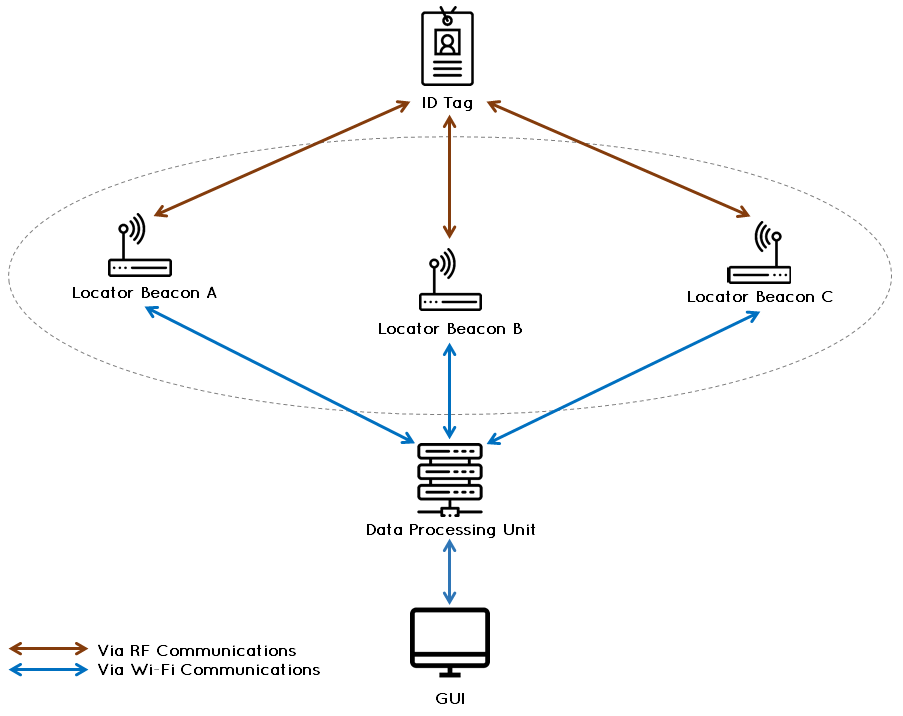
\includegraphics[scale=0.65]{./images/00_sys_arch.png}
    \caption{High Level System Layout}
    \label{sys_arch}
\end{figure}



\pagebreak
\subsection{Proof of Concept}
\medskip
The Proof of concept phase demonstrates the feasibility and functionality of an indoor location determination system. The PoC system will evaluate how effect a trilateration method is to determine the distance and location of a mobile  ID tag in two dimensional space as well as to establish an initial development system. Similar to the system block diagram shown in figure \ref{poc}.

\bigskip
ESP32 micro-controllers are used as the main hardware components of the Beacon and ID Tags. The ESP32 is an off the shelf, low-cost, low-power system on a chip micro-controllers with integrated Wi-Fi and dual-mode Bluetooth. Received Signal Strength Indicator (RSSI) from Bluetooth Low Energy (BLE) modules are used to estimate distance between each beacon and ID tag. Each beacon determines the MAC address and a RSSI measurement from the advertising ID Tag. The data is forwarded to the data processing unit - Raspberry Pi, via USB serial communication. The RSSI is then used to estimate distance between each ID Tag and the associating Beacon and the results are output to a simple UI. 

\medskip
\begin{figure}[H]
\centering
    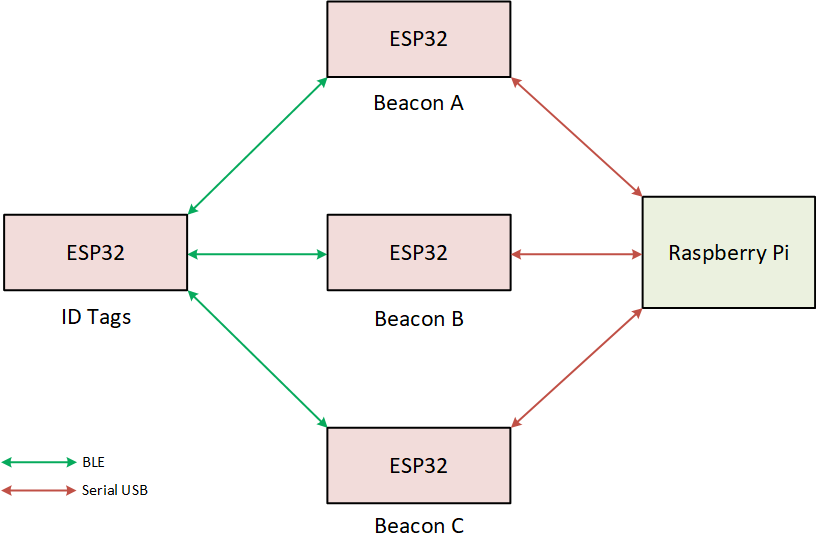
\includegraphics[width=\linewidth]{./images/01_poc.png}
    \caption{PoC System Block Diagram}
    \label{poc}
\end{figure}



\pagebreak
\subsection{Prototype}
\medskip
In the Prototype development phase the transceivers will be incorporated with Decawave DWM1000 UWB modules. The DWM1000 UWB uses radio frequencies in the range of 3.5 to 6.5 GHz; this would significantly reduce issues of signal interference or multipath propagation which would occur by using RSSI with BLE. The DWM1000 will be incorporated as the transceiver with the ESP32 as the main MCU as shown in figure \ref{prototype} below. RF data communication functions will be established between four UWB modules with one as the ID Tag and three as the Locator Beacons to demonstrate distance estimation with DWM1000 UWB modules. This will be achieved by using signal fingerprinting to determine transmitter properties such as ToF and unique Tag identifier. Furthermore, trilateration algorithms will be implemented on data processing unit to determine near real time location and coordinates of ID Tags. Initial Implementation of software stack on data processing unit and development of GUI will occur during this phase as well.

\medskip
\begin{figure}[H]
\centering
    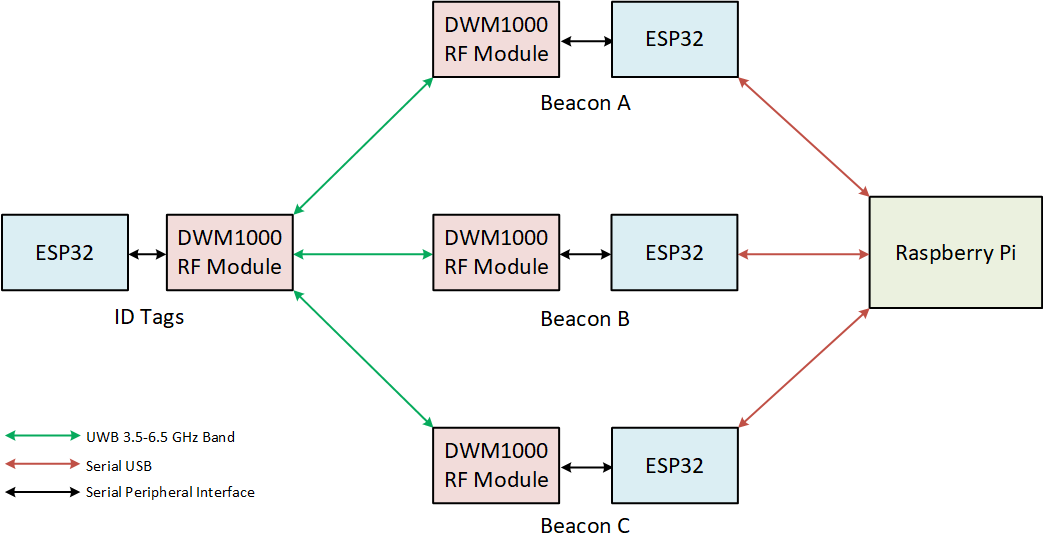
\includegraphics[width=\linewidth]{./images/02_prototype.png}
    \caption{Prototype System Block Diagram}
    \label{prototype}
\end{figure}


\pagebreak
\subsection{Final Product}
\medskip
The final product will demonstrate the fully functional indoor rescue system that detects the location of the ID tags and displays it accordingly on a GUI. Here the addition of ESP32’s Wi-Fi modules can be seen (Figure \ref{final}), as the Beacon will communicate via Wi-Fi communication with the data processing unit. The Wi-Fi network will be a closed network meaning that the network is only share between beacons and the data processing unit to ensure security, reliability and stability. Furthermore, implementation of RF harvesting circuit for ID Tag device charging during deep sleep mode will occur during this stage. All the components of the systems will be fully integrated as a close-to-production product. Component circuits and PCB footprint will be minimized and proper casing will be made to house all electronics. The data processing unit will provide the user with a full GUI to interact with the system along with the fully implemented features such as importable blueprints and multi-floor tracking.

\medskip
\begin{figure}[H]
\centering
    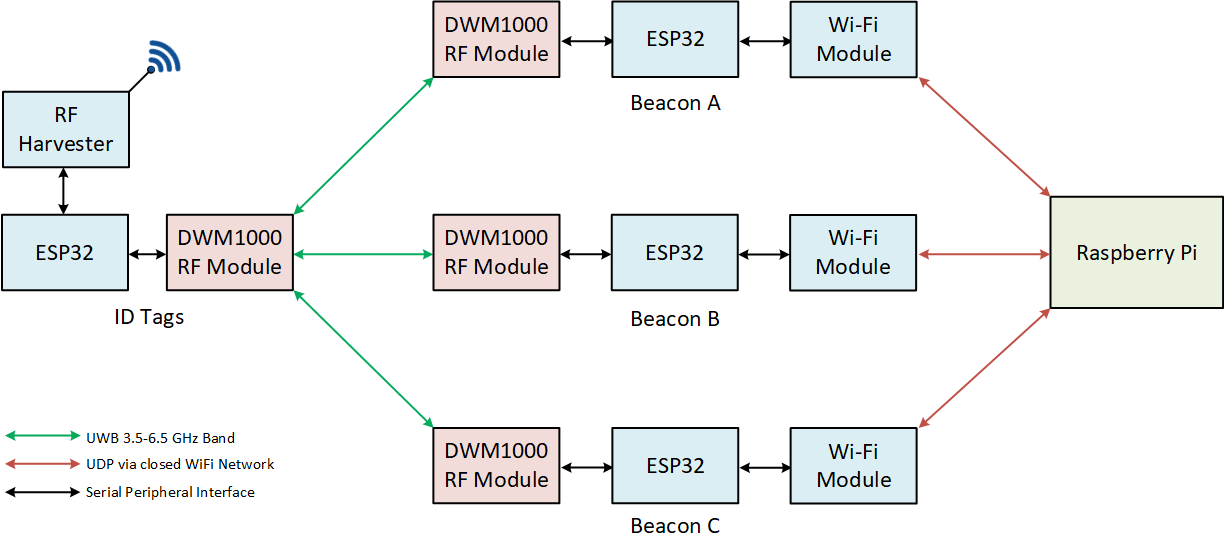
\includegraphics[width=\linewidth]{./images/03_final.png}
    \caption{Final System Block Diagram}
    \label{final}
\end{figure}




\pagebreak
\subsection{Ultra-Wideband Radio Technology}
\medskip



\pagebreak
\subsection{Trilateration Methods}



\pagebreak


\setcounter{section}{2}
\section{System Components}
\bigskip

\subsection{MCU - ESP32}
\medskip
ESP32 is a series of low-cost, low-power system on a chip microcontrollers with integrated Wi-Fi and dual-mode Bluetooth. Created and developed by Espressif, the ESP32 contains a Tensilica Xtensa LX6 microprocessor in both dual-core and single-core variations and includes a in-built antenna, power amplifier, low-noise receive amplifier, filters, and power-management modules (As shown in figure \ref{esp_core}) \cite{R3-1-1}. 

\medskip
\begin{figure}[H]
\centering
    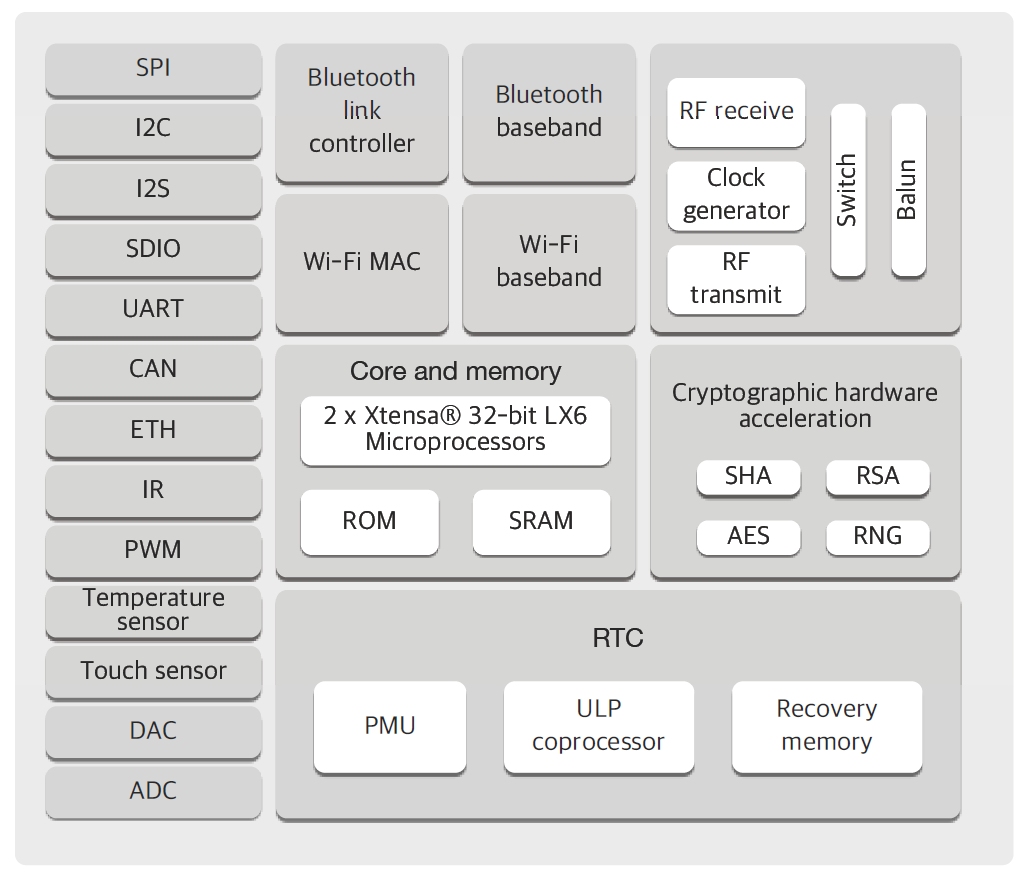
\includegraphics[scale=0.4]{./images/esp_core.png}
    \caption{ESP32 Architect Block Diagram}
    \label{esp_core}
\end{figure}

For the proof of concept, the Bluetooth modules on the ESP32 will be used as the communication interface between the Beacon and the ID tags. Using BLE advertising, the ID Tags ESP32 broadcasts a unique MAC address. The Beacon ESP32 can collect all assicating ID Tag ESP32s and capture the RSSI and MAC of these devices. These information are forwarded to the DPU for distances establition and location plotting.

\begin{figure}[H]
\centering
    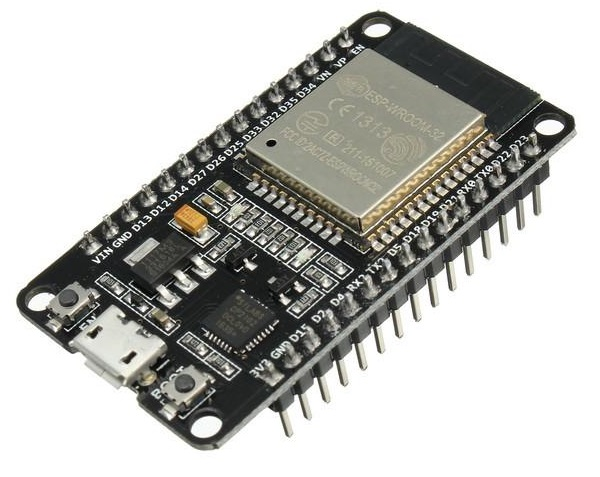
\includegraphics[scale=0.25]{./images/esp.jpg}
    \caption{ESP32 Development Board}
    \label{esp}
\end{figure}


\pagebreak
In the Final design the ESP32 will be incorporated as the main controller unit for both the beacons and ID tags but with Decawave DWM1000 UWB modules as the transceiver. For the beacons the ESP32’s Serial Peripheral Interface (SPI) will be used to interact with the Decawave DWM1000 UWB modules. As for the ID Tags, the ESP32 features a deep sleep mode which reduces power consumption to about 10uA from 260mA (active operations), thus drastically increasing the battery life time. Furthermore, with its wide range of capabilities such as Wi-FI and Bluetooth, a mesh network and be implemented to extend the communication range of the Beacons. A mock-up circuit diagram presenting the SPI interface between the ESP32 and a breakout board for DWM1000 is shown in figure \ref{eps_dwm_circuit}.

\medskip
\begin{figure}[H]
\centering
    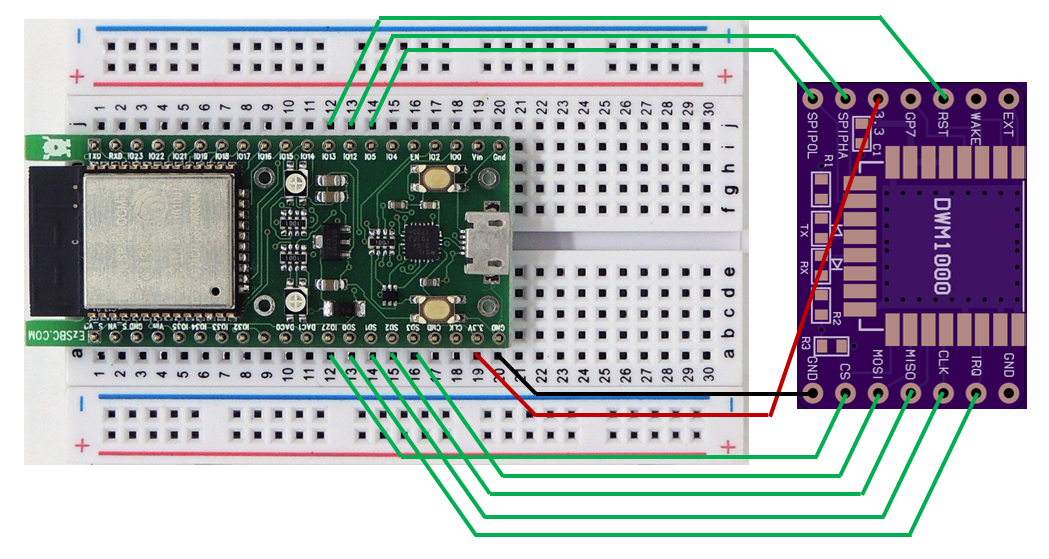
\includegraphics[scale=0.5]{./images/eps_dwm_circuit.png}
    \caption{Circuit Diagram of ESP32 \& DWM1000}
    \label{eps_dwm_circuit}
\end{figure}



\pagebreak
\subsection{Transceiver - DWM1000} 
\medskip
The Beacon and ID Tag communication will be done using ultra-wideband wireless communication. The most optimal transceiver available on the market that most fits the needs and scope of this project is the Decawave DWM1000 UWB module (Figure \ref{dwm1000}). The DWM1000 is an IEEE802.15.4-2011 UWB compliant and FCC/ETSI certified wireless transceiver module based on Decawave’s DW1000 IC \cite{R4-2-1}. This module is a combination of DW1000 IC, a built in antenna, power management system, and clock control for simple design integrations (Figure \ref{dwm1000_bd}). 

\medskip
\begin{figure}[H]
\centering
    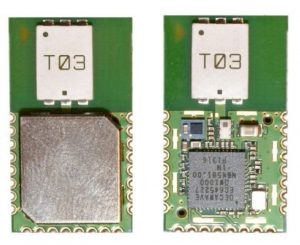
\includegraphics[scale=0.75]{./images/dwm1000.jpg}
    \caption{Decawave DWM1000 Modules}
    \label{dwm1000}
\end{figure}

The module enables the location tracking of objects in real time location systems (RTLS) to a precision of 10 cm indoors. It supports high range of communications data rates from 110 Kbps up to 6.8 Mbps, with excellent communication ranges of up to 300m. The frequencies of operation in the range of 3.5 GHz to 6.5 GHz with seven distinct channels which would significantly reduce issues of signal interference or multipath propagation. Its small physical size allows the module to be implemented in highly cost-effective solutions. By using this modul,e integration with the Akriveia Beacon system is intuitive and simple; since the DWM1000 also offers a wide range of MCU support such as Arduino MCUs or the ESP32 MCUs. 

\medskip
\begin{figure}[H]
\centering
    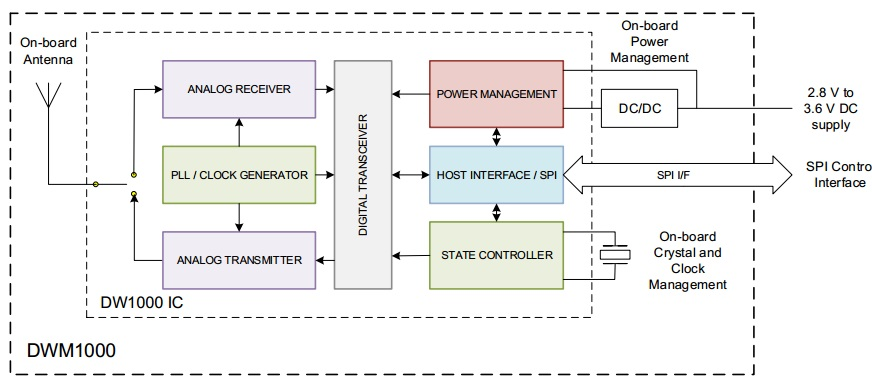
\includegraphics[scale=0.7]{./images/dwm1000_bd.jpg}
    \caption{DWM1000 Internal Block Diagram}
    \label{dwm1000_bd}
\end{figure}



\pagebreak
\subsection{DPU - Raspberry Pi}
\medskip
The Data Processing Unit is a stand alone single board computer (SBC). For the demonstration of this project a Raspberry Pi 3 B+ is used as the DPU since it is an affordable and robust SBC, but the DPU in theory should be any electrical computer device that is capable of running a basic linux operating system; as the software stack is designed to operate on any linux based system. Since the Pi is cheap, portable and designed with an Cortex-A53 processor it meets the minimum requirements for the DPU.

\bigskip
The Raspberry Pi 3 B+ is a single board computer with a 1.4GHz 64-bit quad-core processor, dual-band wireless LAN, and Bluetooth 4.2/BLE \cite{R3-3-1}. The Broadcom BCM2837B0, Cortex-A53 (ARMv8) 64-bit SoC at 1.4GHz quad-core processor allows complex tri or multilateration calculations done simultaneously for multiple ID Tags. With dual-band 2.4GHz and 5GHz IEEE 802.11.b/g/n/ac wireless LAN, the Pi can create a reliable network access for multiple ESP32 for data forwarding. At a power rating of 5V/2.5A DC the Pi requires minimal power to operate, which allows for a variety of power options during emergency disasters. Furthermore, the Pi is configured with a linux based OS, Debian which contains the software stack developed in Rust that will create a layer of user interface between the user and the Akriveia Beacon system.


\medskip
\begin{figure}[H]
\centering
    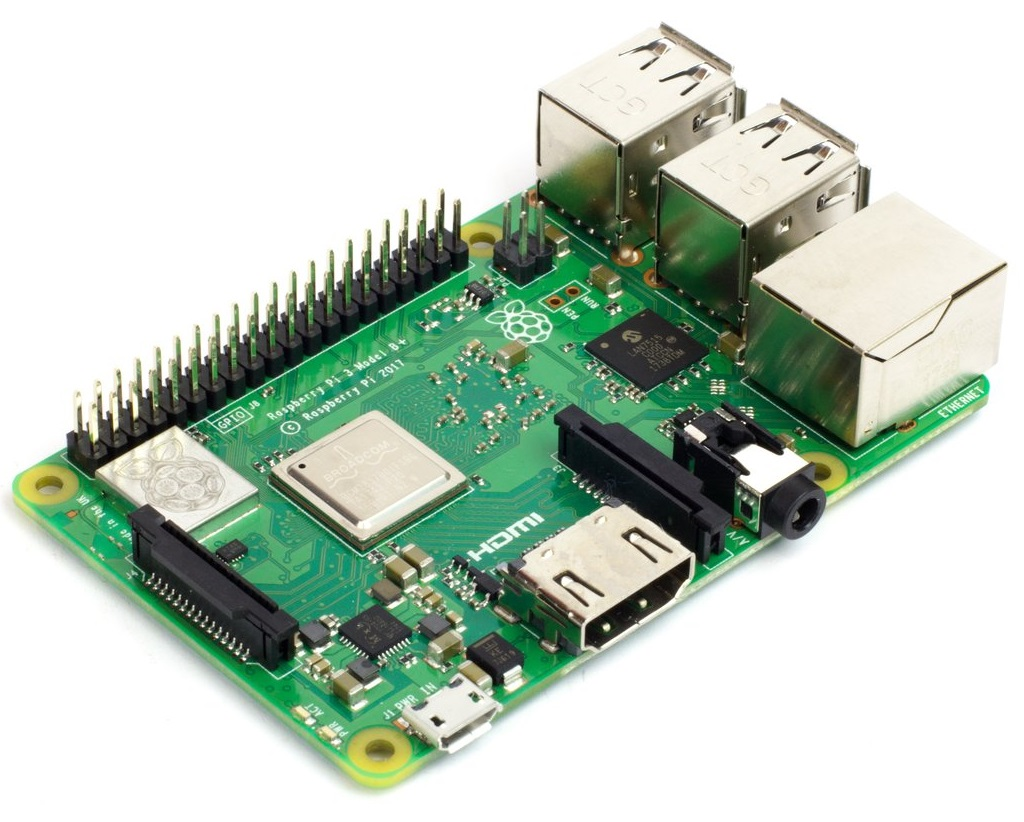
\includegraphics[scale=1]{./images/pi.jpg}
    \caption{Raspberry Pi 3 B+ Model}
    \label{pi}
\end{figure}





\pagebreak


\setcounter{section}{3}
\section{Hardware Design}
\bigskip
\subsection{System Operation Modes}
\medskip
The Akrievia Beacon system will have two modes of operations, the idle mode, and the emergency mode. Idle mode occurs during every day operation that is not under an emergency. An emergency is defined as a situation that poses an immediate risk to health, life, property, or environment. Most emergencies require urgent intervention to prevent a worsening of the situation. In emergency situations the system will be triggered on to operate under the emergency mode following a system state diagram as shown in figure \ref{sys_state}.

\bigskip
When system is under idle mode, the beacon system does not attempt to transmit location information from ID Tags to the DPU, as the ID Tags will be under deep sleep mode. In idle mode the system is available for configuration such as adding/deleting ID Tags and beacons. In the Event of an emergency, a trigger such as one that could be associated with a fire alarm will trigger the system state into the emergency mode.

\bigskip
When system is under emergency mode, the beacons will attempt to establish a data pipeline using the UWB modules. And the ID Tags are triggered on by personnel carrying the device that are in need of rescue or assistance. Under emergency mode the DPU triggers the Beacons to start sending and receiving packets to determine ToF data from the ID Tags. The ID tags will receive request packet from beacon and transmit location data back to the beacon. Once the emergency situation is resolved the system can be switched back into idle mode.

\medskip
\begin{figure}[H]
\centering
    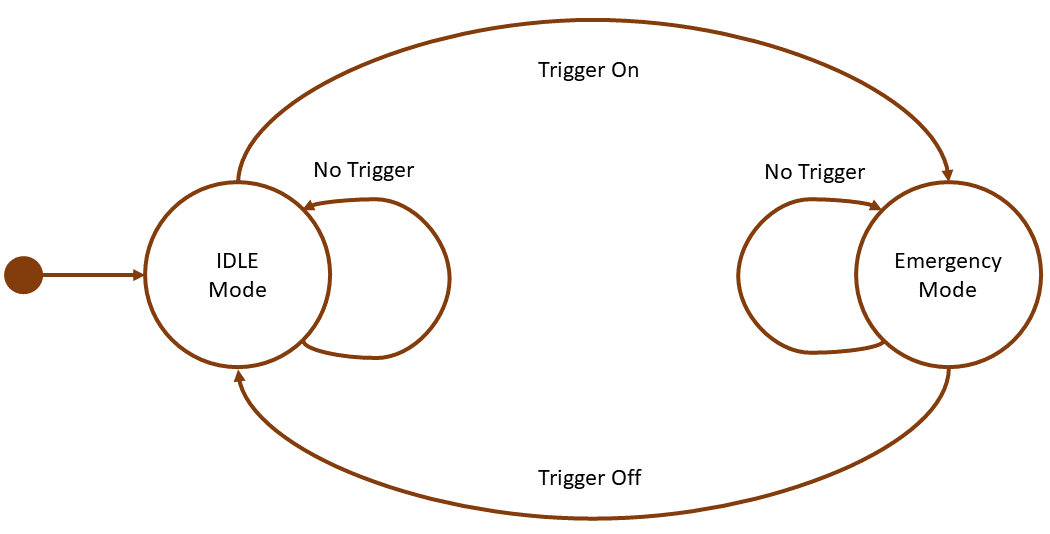
\includegraphics[scale=0.6]{./images/state_d.png}
    \caption{Akriveia Beacon System State Diagram}
    \label{sys_state}
\end{figure}
\medskip



\pagebreak
\subsection{Communication Protocol}
\subsubsection{Beacon to ID Tag Communication}



\pagebreak
\subsubsection{Beacon to DPU Communication}
\medskip
For the proof of concept and prototype, data-pipeline is a simple implementation with USB serial interface. The Beacon and DPU  will listen and send data with the data processing unit over the serial read and write interface. 

\bigskip
In the Final design the Beacons will use the WiFi module on the ESP32 to join a privately hosted access point created by a hostapd on the data processing unit (Raspberry Pi). Once each beacon is connected to the access point they will be assigned an IP by the Dynamic Host Configuration Protocol (DHCP) server. A one-to-many network will be created as shown in figure \ref{udp}. Using User Datagram Protocol (UDP) communication over the networking layer, the DPU can bind on the gateway IP and a specific port to listen for forwarded beacon data. To initiate control with the beacons, the DPU will bind to each beacon IP at a specified port and send commands using UDP.

\medskip
\begin{figure}[H]
\centering
    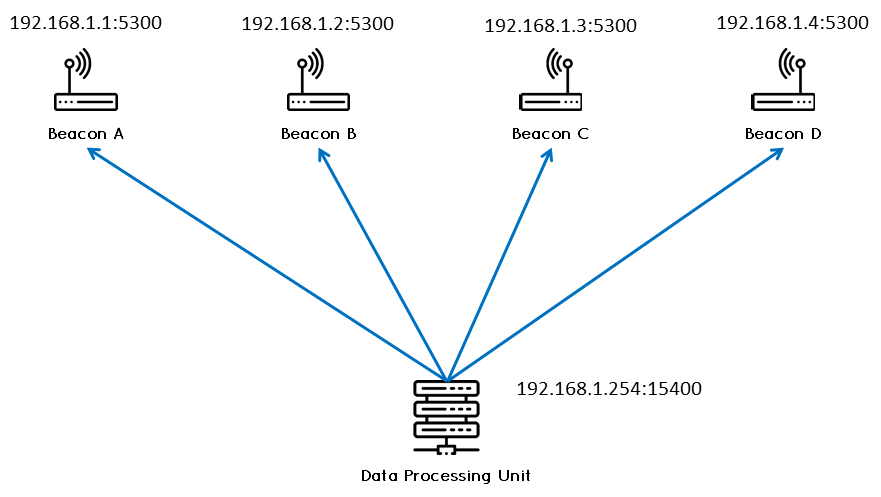
\includegraphics[scale=0.7]{./images/UDP.png}
    \caption{UDP Communication Network}
    \label{udp}
\end{figure}
\medskip



\pagebreak
\subsection{Beacon Design}
The Beacon units, which will relay location data from the ID Tags to the Data Processing Unit (DPU), consist of an ESP32 module, a DWM1000 UWB transceiver, a 9V lithium ion battery, and a power cable. These components will be contained in an encasing made from PLA plastic. This unit will have LEDs indicating the power state, and whether the Beacon is transmitting or receiving, and a reset button. The DPU will send a command to the beacon and the ESP32 will evaluate the command and execute accordingly as shown in figure \ref{bcn_flow}.

\medskip
\begin{figure}[H]
\centering
    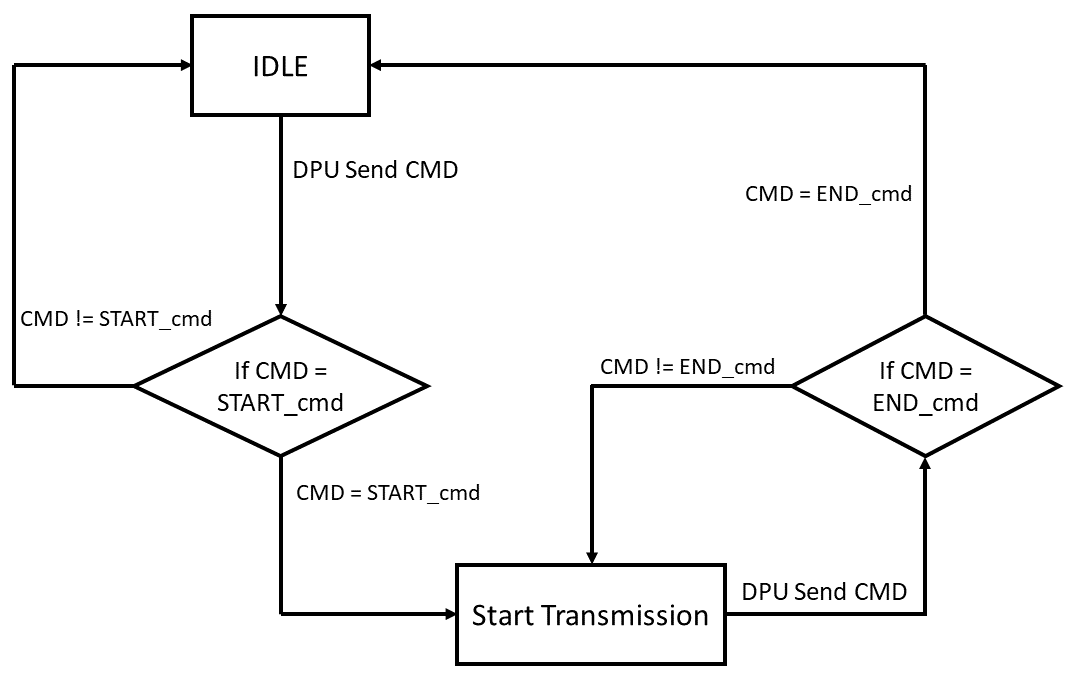
\includegraphics[scale=0.40]{./images/beacon_flow.png}
    \caption{Beacon System Flow Diagram}
    \label{bcn_flow}
\end{figure}
\medskip

A 3D appearance mock-ups of the ID Tag was done in Solidworks and can be seen in the Computer Aided Design (CAD) representation, figure \ref{Bcn_CAD}. 

\medskip
\begin{figure}[H]
\centering
    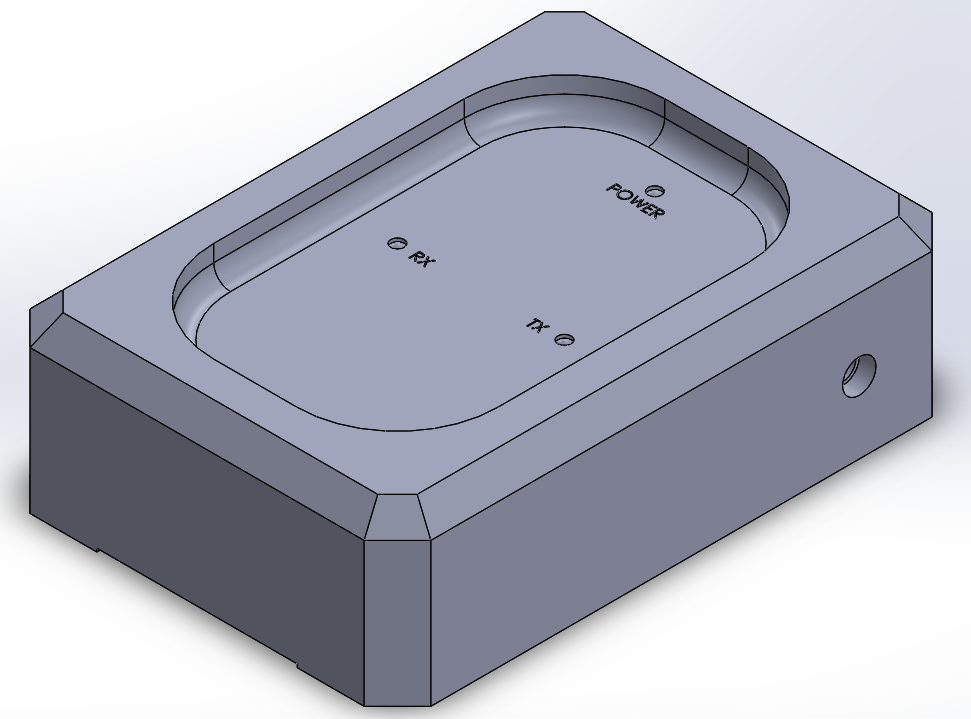
\includegraphics[scale=0.40]{./images/Beacon.png}
    \caption{CAD representation of Beacon}
    \label{Bcn_CAD}
\end{figure}



\pagebreak
\subsection{ID Tag Design}
The ID Tags, the part of the system being tracked by the Beacons, will be powered by a rechargeable 4.5 V battery, which will be charged over time by a RF harvester (see sec. 5.2). The ID Tag will consist of an ESP32 MCU module, and a DWM1000 UWB transceiver chip. The ESP32 is used in the ID tag as it has a function called deep sleep mode, in which the ID Tag has minimum power consumption and does not transmit data for  location tracking. The ID Tag will be activated in an emergency situation via capacitive touch button on the unit. If the button is pressed, and the system is not in an emergency state, the ID Tag will show the charge level and return to deep sleep. However if there is an emergency the ID Tag will then transmit a ping back to the beacon to produce location data as described in the system flow diagram in figure \ref{id_flow}. 

\medskip
\begin{figure}[H]
\centering
    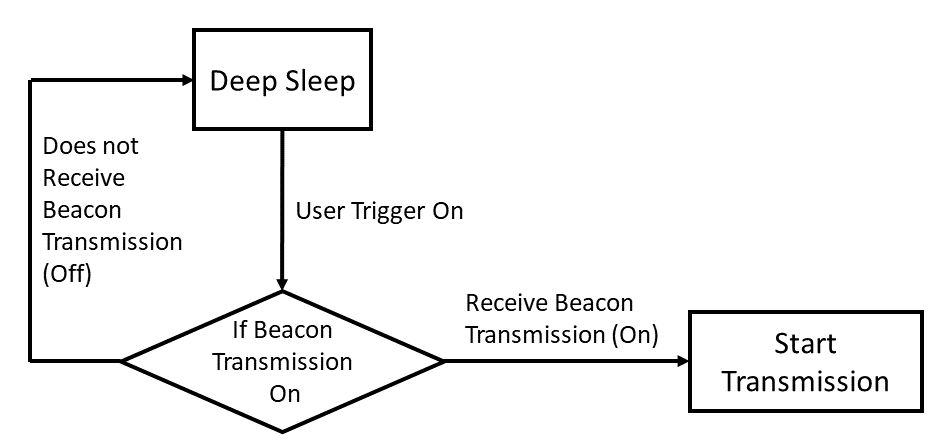
\includegraphics[scale=0.50]{./images/id_flow.png}
    \caption{ID Tag System Flow Diagram}
    \label{id_flow}
\end{figure}
\medskip

A 3D appearance mock-ups of the ID Tag was done in Solidworks and can be seen in the CAD representation, figure \ref{ID_Tag}. The internal components of the ID Tag will be contained in a PLA plastic shell with LEDs indicating the power state, transmission activity, and charge level of the ID Tag. 

\medskip
\begin{figure}[H]
\centering
    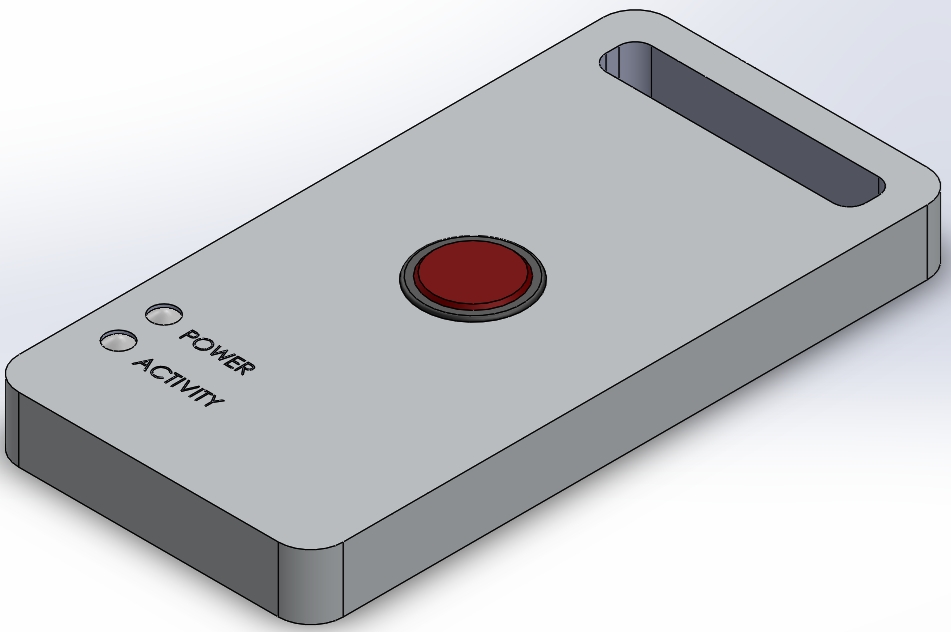
\includegraphics[scale=0.40]{./images/ID_Tag.png}
    \caption{CAD representation of ID Tag}
    \label{ID_Tag}
\end{figure}



\pagebreak
\subsection{Hardware Design Specification}
\medskip
TRIWAVE SYSTEMS has chosen to develop the proof-of-concept prototype using 2.4 GHz Bluetooth radio modules as feasibility testing, before upgrading the system to using Decawave DWM1000 Ultra-Wideband (UWB) modules for further prototyping. ESP32 Micro-controller Units (MCUs) will be used to control the beacons and ID tags and a Raspberry Pi 3 B+ will be used as a data processing unit. The requirements below detail the requirement for hardware functionality of the Akrivia Beacon system.
\medskip
\bgroup
\def\arraystretch{1.5}
\begin{table}[H]
\centering
\begin{tabular}{ | m{3cm} | m{12.5cm} |}
\hline
\textbf{REQ.HW.1 - C} & The Beacons must use ESP32 as the microcontroller unit and transceiver \\
\hline
\textbf{REQ.HW.2 - C} & The ID Tag must use ESP32 as the microcontroller unit and transceiver \\
\hline
\textbf{REQ.HW.3 - P} & ID tag broadcast duration must be at least 1 hour long upon activation\\
\hline
\textbf{REQ.HW.4 - P} & ID tag must return to deep sleep mode after broadcasting period\\
\hline
\textbf{REQ.HW.5 - P} & The Beacons must use Decawave DWM1000 UWB modules as transceivers\\
\hline
\textbf{REQ.HW.6 - P} & The Beacons must use ESP32 as the controller units\\
\hline
\textbf{REQ.HW.7 - P} & The ID tags must use Decawave DWM1000 UWB modules as transceivers\\
\hline
\textbf{REQ.HW.8 - P} & The ID tags must use ESP32 as the controller units\\
\hline
\end{tabular}
\caption{Hardware Design Specification}
\end{table}








\pagebreak


\setcounter{section}{4}
\section{Electrical Design}
\bigskip


\pagebreak


\setcounter{section}{5}
\section{Software Design}
\bigskip

% NOTE: future work would be to build a system to flash new beacons with firmware for the credentials to communicate with the system.
% NOTE: assume beacons have line of sight to eachother. this allows us to make the callibration phase easier by manually measuring the distance between beacons rather than creating a callibration script.

%Libraries/Packages/Frameworks
%Software Stack

% discuss the system at a high level, but leave details to subsections
% breifly reintroduce important topics that the user will need to be reminded of
\subsection{Software Overview}
% TODO revise
The Akriveia system is comprised of 3 different devices, namely: the data processor, beacons, and id tags; this device diversity plays a large role in the software choice for the beacons and id tags.
\smallskip
The Akriveia data processor is the primary access point for Administrators and First Responders, of whom will be presented a Graphical User Interface served by the data processor in addition to handling commands from the client.
The software on the server is written entirely in rust, including the static client side webpage.



\smallskip
The requirements for each device are different, however the id tags and beacons are able to share a similar environment.
As such Akriveia will require two different software environments.

\bigskip
% language choices, formatting, standards, libraries
\subsection{Software Stack}
Akrivia is composed of two primary languages, the server is implemented entirely in rust while the beacons and id tags use C++.

\bigskip
\subsubsection{Software Environments}
The data processing server requires an operating system to perform mundane CPU scheduling for our multithreaded application, wifi drivers, and a proper file system to handle a database.
As such, the linux - and more specifically the debian destribution of linux - was chosen as the servers operating system.

\bigskip
% TODO add a citation for debian stability
Debian is widely praised for its stability, which makes it ideal for a data processing server because Akriveia simply cannot fail as lives depend on it to work.
Debian brings in the aptitude package manager for dependency management, which allows for quick installation of required driver updates, operating system updates, and any additional packages required by Akriveia.
Debian's Aptitude has the advantage compared to other package managers because it removes the need to worry about dependencies, manual installation, and even installation of sub dependencies.
As Debian is a linux distribution, it has widespread hardware adoption across many different hardware architectures - primarily x86-84 and ARM64 - giving Akriveia the flexibility to run almost anywhere with little cost.

\bigskip
Debian is contrasted by another linux distribution called arch linux which uses a different package management paradigm called rolling releases, favoring earlier adoption of newer packages to more quickly introduce features at the cost of stability.
Another alternative to Debian is Windows, however Windows suffers from high power usage, poor package management, and heavy reliance on proprietary software, whereas linux is free of cost, open source, and has a more inclusive licence.

\bigskip
\subsubsection{Software Languages}
% TODO revise with word flow in mind. segmented thoughts in each sentence.
The server is written in rust.
% TODO make the citation work
Rust is a newer language compared to C, it was created in 2006 \cite{rust_graydon_interview} and its first stable version was released in 2015 \cite{rust_releases}, taking inspiration from C++ and Haskell in its design.
Rust is a systems language designed for stability and robustness, it eliminates entire classes of errors using its borrow checking system, a feature unique to this language.
The borrow checking system defines a strict set of rules to follow, and fails to compile if these rules are broken - even if the application is otherwise logically correct.
As a systems language, rust is compiled to binary rather than executed as a script through an interpreter however this does not stop it from being a higher order language.
The borrow checker statically analyzes the code being compiled, and in doing so is able to statically determine when to allocate and more importantly when to free heap allocated memory.
Fundamentally, this means that without a garbage collector and without manually managing memory, rust provides a mechanism to manage memory without a runtime cost while behaving like a garbage collected language providing great flexibility in expressiveness and allowing higher order operations without taking brain resources.

\bigskip
The beacon and id tag are written in C++.
Ideally, the entire project would be written in one languge, however for the case of programming embedded devices, namely arduinos, we have opted to stick wih the standard toolset shipped with the arduino tools.
C++ is specifically designed for embedded programming, allowing use of higher level features when desired while also giving the developer absolute control over how memory is managed.
On arduinos, memory is very limited so control is key to fitting our program within the small space constraints.


\bigskip
\subsubsection{Software Standards}
% TODO references here
Rust code will follow the the rustfmt standard of source layouts, rustfmt is a tool provided by the rust project that automatically formats all source in the standard format. The rust compiler also provides a few warnings for common formatting issues builtin, which will be heeded.

\bigskip
C++ will follow the iso C++ programming standards \cite{cpp_core_guidelines}. The arduino style guide \cite{arduino_style_guide} was also considered, however the rules list they present is incomplete and more ad hoc than a full style guide.

% introduce major libraries that largely dictate how we implement the system.
\subsubsection{Frameworks}
Akriveia's main server framework is called Actix.
Actix is an Actor Framework that follows the Actor Model paradigm of multithreaded workloads.
The Actor Model operates on objects called actors to orchestrate concurrent computations, it does this by treating actors as seperate entities that execute on an event loop on one or more threads, where the event loop simply looks at a list of events generated by actors and executes each event in order as long as it is not blocked by other events.
Events are generated when actors pass messages to eachother, in response the actor that receives the message can modify its local state, create other actors, send messages to other actors, execute arbitrary logic, and finally send a response to the message.
This programming paradigm prevents the need for locks (and by extension, deadlocks) because the message passing mechanism alleviates the need to manually manage concurrency, opting to use atomics instead.
\bigskip
Actix was chosen as the primarily to give the flexibility of multithreading without incurring the typical thought process overhead associated with multithreading. Additionally, as a framework rather than a library, Actix serves as the basis to make REST webservers through the package Actix Web, which is further discussed under the \ref{software_libraries} section.

% discuss which libraries we are using, and how they will be used by us
\subsubsection{Libraries}
\label{software_libraries}

\begin{table}[H]
\centering
\begin{tabular}{ | m{3.25cm} | m{12.5cm} |}
	\hline
	\textbf{Actix Web} & The Actix Web library is a crate that extends the functionality of the Actix framework to create HTTP webservers. \\
	\hline
	\textbf{Yew} & Yew is a crate that extends Rusts ability to compile to Web Assembly by adding the ability to dynamically generate html on the client in response to user events and server responses. This library is very similar to Facebook's React for javascript. \\
	\hline
	\textbf{Serial Port} & Enables serial communication over USB between the server and beacons.\\
	\hline
	\textbf{Rust Standard Libraries} & This is the standard Rust runtime library, and contains many useful boilerplate functions and generic types. This library is included with the basic installation of rustc. \\
	\hline
\end{tabular}
\caption{Akriveia Dependencies - Rust}
\end{table}

\begin{table}[H]
\centering
\begin{tabular}{ | m{3.25cm} | m{12.5cm} |}
	\hline
	\textbf{Arduino Runtime} & This is the standard set of arduino runtime libraries based off of the clib standard library tailored specifically for Atmel Atmega microcontroller chips. \\
	\hline
	% TODO wifi library
\end{tabular}
\caption{Akriveia Dependencies - C++}
\end{table}

\bigskip
% discuss the model view controller paradigm, and its benefits
\subsection{Model-View-Controller}
% TODO glossary of mvc
The model-view-controller(MVC) paradigm is a common method of seperating concerns between modules.
It is an architectural pattern that seperates concerns in a general way, allowing for code reused and improving parallel developement, it is also a common practice which allows others familiar with the paradigm to ramp up quickly on the project.
The model describes data, data manipulation, as well as data storage.
The view simply describes how to view the model.
The controller acts as the means to communicate between the view and model based on data inputs, and is also capable of higher order operations such as between multiple models.

\bigskip
As the Actix Web library is less mature than frameworks in other languages such as Python's Django or Ruby's Rails, Akriveia's data processor will be an implementation of a large portion of manual MVC boilerplate.
This allows for greater flexibility in implementation, at the cost of marginally higher developement time.
A benefit is that MVC does not have a good answer for funcitonality that falls outside of the architectures coverage such as background tasks.
Akriveia is required to maintain communication with many beacons and perform calculations asyncronously from web requests, which is the perfect usecase for the actor framework which fills the void of the model-view-controller.


\bigskip
% discuss how we plan to multithread the data processor. go into slightly more detail about actix actors, and why this
% is necessary
\subsection{Threading Model}
The purpose of multithreading the DPU is to make use of the hardware provided, since all modern server and desktop processors have at least two dedicated hardware cores.
Additionally, it is important for the DPU to have realtime responsiveness on the webserver, requiring that large computations such as triangluation for many beacons must be offloaded to other threads, keeping responsiveness high since the webserver thread is not blocked on computation while a request comes in.
An additional consideration specifically for the proof of concept which uses blocking serial communication to communicate to the beacons, meaning that each beacon requires a dedicated thread to communicate with the DPU.

Rust and Actix make multithreaded development easier by using message passing for interthread communication, at the cost of performance when compared to traditional mutexes and atomics.
The implementation of message passing is a thread safe queue using mutexes and atomics to ensure data integrity, where multiple threads are able to send commands to another thread, which recieve the message without blocking either thread.
To further discuss the Actix threading model, some definitions are required:
\begin{enumerate}
	\item Actor: A class that contains message handler callbacks.
	\item Arbitor: A thread pool, where each thread in the pool is an event loop.
\end{enumerate}
Once instantiated, the arbitor spawns as many threads as indicated by its constructor and waits for actors to be spawned within the thread pool.
By default, the number of threads in the pool is the number of cores on the CPU.
The arbiter is an environment for actors to execute, and as actors are spawned into the thread pool, they can send messages to other actors, or create other actors in response to external events such as from the file system or HTTP requests.
As shown in Figure~\ref{actix_thread_model}, the arbitor manages its own threads, which are all spawned at startup rather than on demand.
Within each thread, the arbitor executes the event loop, which polls its queue, and acts on any messages in the queue by delegating the task to the actor the message is bound to.
To pass a message to another actor, the sender must have the address of the recipient so that the arbitor can determine the destination, rather than a broadcasting system; this is shown in Figure~\ref{actix_messages}.

\begin{figure}[H]
	\centering
    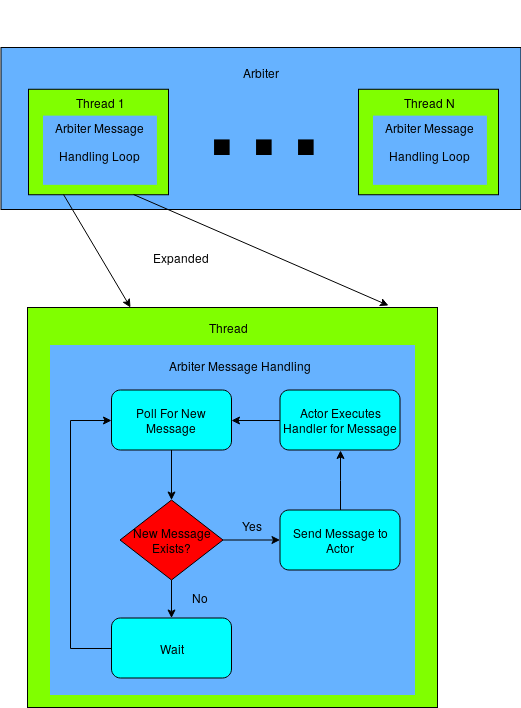
\includegraphics[scale=0.6]{images/actix_thread_model.png}
    \caption{Actix Thread Model}
    \label{actix_thread_model}
\end{figure}
\begin{figure}[H]
	\centering
    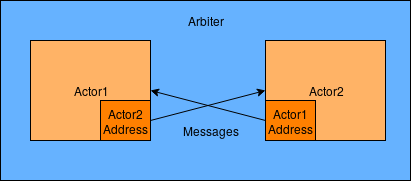
\includegraphics[scale=0.6]{images/actix_message_passing.png}
    \caption{Actix Message Passing}
    \label{actix_messages}
\end{figure}

The beacons and id tags do not have a full OS, so they can only rely on single threaded interrupt handling to "multitask".
Interrupt handling does not provide full concurrency, instead it time slices the single core to provide the illusion of multitasking.
Interrupt handling is calling a function as a result of an event such as an external device raising a bit high on the CPU, or when a timer goes off.
In the Proof concept, the bluetooth library uses this functionality to handle connections.
When transitioning to wifi and UWB, similar functionality will be implemented in each respective technology's library, of which Akrievia simply relies on rather than reimplementing ourselves.

\bigskip
% discuss the data processor subsystems in detail
\subsection{Data Processor Software Architecture}
In the proof of concept, the DPU creates an HTTP server actor and a beacon manager actor.
The HTTP server waits on web requests, delegating tasks to the beacon manager and polling it for the necessary information.
On startup, the beacon manager queries the number of serial arduino devices, spawning a thread for each device.
Each thread spawned by the beacon manager represents a serial connection to a beacon.
The beacon manager sends messages using a traditional Multiple Producer Single Consumer Message Queue (MSPC) defined in the rust standard library, while the each serial communcation thread returns messages back to the manager through the actix message passing system.
Figure~\ref{software_poc_arch} gives a graphical representation of the previous description.
As a side note, Actix uses MSPC internally for its message passing system.

\bigskip
The prototype and final versions bring in major changes to the software design.
As shown in figure~\ref{software_final_arch}, a major change is the removal of the serial connection actor which is replaced with the udp actor(which tentatively may be tcp instead).
The beacon manager remains, but instead controls the udp actor rather than the serial connections.
An additional role of the beacon manager is to delegate computation of triangulation to the triangulation processor actor, which will save data in memory until there are at least 3 data points for a single it tag to determine its position.
The triangluation processor makes the positional calculation and saves new position to disk via the id tag model, which abstracts the database query.
The beacon and map models perform a similar role, abstracting their associated database queries into a single location following MVC.
Controllers mainly handle the model they were paired with, however the id tag controller will also query the triangulation processor for realtime positional data and the beacon controller commands beacons indirectly through the beacon manager.

\begin{figure}[H]
	\centering
    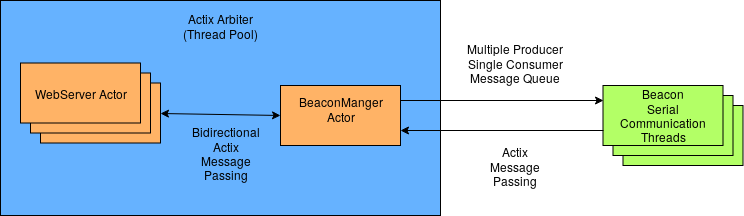
\includegraphics[scale=0.6]{images/poc_arch.png}
    \caption{Proof of Concept Software Architecture}
    \label{software_poc_arch}
\end{figure}

\begin{figure}[H]
	\centering
    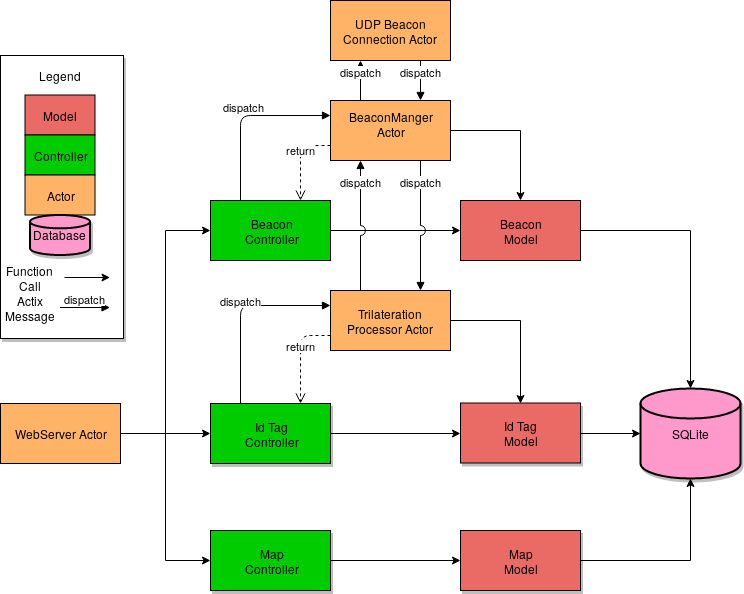
\includegraphics[scale=0.6]{images/prototype_software_arch.png}
    \caption{Final Software Architecture}
    \label{software_final_arch}
\end{figure}

\bigskip
% discus the purpose of the webserver, and how it will be used to control the other subsystems dictated by user command.
\subsubsection{Webserver Subsystem}
The purpose of the Webserver Subsystem is to bridge the GUI and backend by providing a data transfer interface in the form of HTTP REST calls.
A Webserver architecture is chosen because of its simplicity to implement, widespread adoption, and flexibility.

\bigskip
The Webserver Subsystem will be designed to serve data to a browser, including the the HTML and Javascript files(GUI files) that are displayed by the browser.
Once the browser has the GUI files, it will make addiitonal requests to the backend to keep updated information displayed on the GUI.
The Webserver Subsystem will only allow logged in users to access sensitive data, and only if they have the correct access rights.
Electron applications and traditional rendering APIs were also considered, however they each have tradeoffs that do not fit with the design requirements of Akrievia.

\bigskip
An electron application that utilizes browser technologies merges the backend and frontend together which will reduce deployment flexibility because a monitor connected directly to the DPU will be the only access point to the GUI, however the display will potentially need to be accessed by multiple users at a time, and will introduce high coupling between the frontend display and backend computation.
Electron applications are also highly single threaded, meaning that they will have higher difficulty in utilizing all cores on the CPU.
Electron applications are fixed to using javascript for both processing and display, whereas a webserver fixes the GUI implementation to javascript however the real processing is performed in a more performant language such as Rust which is compiled to native binaries.

\bigskip
Compared to a traditional GUI implemented using graphics driver interfaces such as OpenGL, Vulkan, DirectX, or any higher level libraries that provide interfaces to graphics drivers, a GUI implemented in HTML and Javascript will take much less time to implement because both Javascript and HTML abstract away memory concerns such as pointers, and will never have memory related runtime errors, as guaranteed by the browser.
Browsers have widespread adoption, in every GUI based operating system at least one browser is installed by default, making them widespread and widely used.
Due to widespread adoption, browsers provide the flexibility to display our GUI either on the computer hosting the server itself, or just as easily the GUI can be accessed through another computer at the customers discretion.


% TODO flesh these out into paras
functions of the data processor:
	- collecting data from each beacon
	- sending commands to each beacon

\bigskip
\subsubsection{Beacon Manager Subsystem}
The role of the beacon manager is to aggregate data from the individual beacon connections, and to give an abstraction for external systems that need not concern themselves with communication details, or how many beacons there actually are.
The Beacon Manager is a singleton, which means there is only one of them in the entire system, and has implications on the design of the rest of the system.
The most notable design influence is that the beacon manager can quickly become a bottleneck if it performs too much processing directly, and so to prevent this the beacon manager offloads as much work as it can to other subsystems.

\bigskip
\subsubsection{Serial Beacon Communication Subsystem}
In the proof of concept design, this actor deals with blocking serial communication with dedicated threads to keep the connection alive and to prevent web requests from blocking.
This subsystem will remain as bare bones as possible, because it only serves the purpose of quickly creating a working system and will likely be discarded in future iterations of the DPU.

\bigskip
\subsubsection{Triangulation Processing Subsystem}
In the final design, the triangulation processing subsystem takes in RSSI and time of flight messages from the beacon manager.
The triangulation processor waits until it receives enough datapoints, and once it has 3 datapoints from 3 different beacons for one id tag it can perform a location calculation
While waiting for a full set of data, the incomplete set of data will be stored in a hash table where the mac address of each ID tag is the key and the contents are an array of data points.
Once the array of datapoints hits the threshhold size of 3 from adding a new datapoint the processor can perform the full triangulation calculation.
The triangulation calculation can then be used to update the database entry for the corresponding ID tag by the processor.
To avoid going to the database for realtime updates of the ID tag locations, the ID tag controller will directly query the Triangulation Processor for the most up to date location infromation, reducing latency.

The existance of the Triangulation Processing subsytem is necessary, because the beacon manager will quickly become a bottleneck due to the fact that it is a singleton in a multithreaded system.
As such, the manager should do as little direct processing and blocking operations itself and instead favor offloading the tasks to other subsystems.

\bigskip
\subsubsection{UDP Beacon Communication Subsystem}
In the final design, this actor will communicate with the beacons over the UDP networking protocol.
UDP was chosen because it has less overhead than TCP, and is more suited for realtime applications such as Akriveia.

\bigskip
% discuss database choice - sqlite and why. lead into our models
\subsection{Database details}
Akrievia requires a database to persist map, beacon, and user information.
In the time constraints of Capstone, the database will be a central location for data.
Ideally a production system would support replication of the database to another location, but this is out of scope for the purposes of this course.

\bigskip
SQLite was chosen primarily because of its simplicity to setup and minimal footprint.
Most commonly used in phones and packaged alongside python, SQLite has a stable file format and large userbase, and because of this has built a reputation for not failing.
SQLite is open source, and because of this issues can directly be brought up to the developers along with help from a large amount of experience from the internet due to the large userbase.
Open source projects are also freely available to browse to learn directly from the codebase when necessary.
In Akriveia, the database is accesed through model objects to keep concerns local to a single set of similarily structured files, and to keep reusability up in the codebase.

\bigskip
% discuss how we plan to represent data in the database, tie back to model-view-controller(specifically models, which
% will implement all of the database queries for the controllers to use.
\subsubsection{Models}
Models are used to group database queries and model operations into a single file for each model, increasing reusability of the system.
Akrievia is expected to maintain three different types of models: maps, ID tags, and beacons.
The following tables \ref{user_model}, \ref{beacon_model}, and \ref{map_model} show their expected data entries and their type for each model, along with the purpose of each entry.

\begin{table}[H]
\centering
\begin{tabular}{| m{3cm} | m{3cm} | m{9.5cm} |}
	\hline
	\multicolumn{3}{|c|}{User Model} \\
	\hline
	Data Name & Type & Explanation \\

	\hline
	Coordinates & 2D Vector & Last known location of the user within the map. \\
	\hline
	Emergency Contact & ref:User & Reference to another user as an emergency contact. emergency contacts wont have an employee id or tag id. \\
	\hline
	Employee Id & String & Employee id for each user, optional, may be useful for internal housekeeping of the company that purchases Akriveia. \\
	\hline
	Full Name & String & Human readable name to identify the user on lists. \\
	\hline
	Id Tag Number & 64bit Integer & table key, unique, id for each user. \\
	\hline
	Last Seen Timestamp & Unix Timestamp & Helps to identify if the id tag data is stale. Used to determine if the employee is at work while the disaster occurs. \\
	\hline
	Map ID & ref:Map & Last known map the user was located at. \\
	\hline
	Notes & String & Notes about the user, ie allergies or disabilities, etc. \\
	\hline
	Phone Number & String & Phone number to contact the user. \\
	\hline
	User Type & String & Indicates the type of user, either admin, employee, emergency contact, or first responder. \\
	\hline
\end{tabular}
\caption{User Model}
\label{user_model}
\end{table}

\begin{table}[H]
\centering
\begin{tabular}{ | m{3cm} | m{3cm} | m{9.5cm} |}
	\hline
	\multicolumn{3}{|c|}{Beacon Model} \\
	\hline
	Data Name & Type & Explanation \\

	\hline
	Mac address & String & unique device identifier for beacon, table key.\\
	\hline
	Map id & ref:Map & Reference to a floor/map - this is really just the floor number. Shows the many-to-one relationship between beacons and floors. \\
	\hline
	Name & String & Human readable String for the device. \\
	\hline
	Notes & String & Notes for the beacon such as which room the beacon is located at. \\
	\hline
\end{tabular}
\caption{Beacon Model}
\label{beacon_model}
\end{table}

\begin{table}[H]
\centering
\begin{tabular}{| m{3cm} | m{3cm} | m{9.5cm} |}
	\hline
	\multicolumn{3}{|c|}{Map Model} \\

	\hline
	Data Name & Type & Explanation \\
	\hline
	Name & String & Human readable floor name for gui. \\
	\hline
	Floor number & String & Table key, unique floor number of the map, this is not an integer to accomodate the possibility of odd floor naming conventions. e.g. floor 1A, or basement. \\
	\hline
	Bitmap data & Binary & Bitmap for the floor blueprints to view on the gui. \\
	\hline
\end{tabular}
\caption{Map Model}
\label{map_model}
\end{table}


% discuss what each controller will do - i dont expect this one to be very meaty
\subsection{Controllers}
Controllers are part of the MVC philosophy, unfortunately actix does not directly support the idea of controllers, however this functionality can be implemented manually using Actix Web primitives.
Each controller exposes available operations for the frontend to manipulate data in a controlled and secure manner.
The controller manages data using the models to perform direct manipulations and can aggregate data that cannot otherwise be done by models.
Table~\ref{controllers_table} shows the list of expected controllers in the DPU, one to match each model.

\begin{table}[H]
\centering
\begin{tabular}{| m{3cm} | m{9.5cm} |}
	\hline
	\multicolumn{2}{|c|}{Map Model} \\
	\hline
	Controller Name & Explanation \\
	\hline
	Maps & Handles requests for map operations such as to create, update, delete the map instances. \\
	\hline
	Beacons & Handles requests for beacon operations such as to create, update, delete beacon the model instances. \\
	\hline
	Users & Handles requests for user(id tag) operations such as to create, update and delete user instances. \\
	\hline
\end{tabular}
\caption{Controllers list}
\label{controllers_table}
\end{table}

% describe how the view will work, but dont go into details about the GUI visuals - leaving that for the ui appendix
% mention browser, js, html, rust -> webassembly compile
\subsection{View}
The view is the last component of the MVC philosophy.
The job of the view is to display data in a friendly and easy to use GUI.
In Akriveia, the view is a static webpage served by the Actix Webserver, and is compiled seperately from the backend.
Traditionally, the browser would render HTML and Javascript served by the backend webserver, however in this project the frontend is written entirely in Rust and compiled to a small HTML stub and webassembly which then dynamically generates more HTML for the browser to render.
The Yew crate makes this all possible, which is a Rust package that leverages the webassembly LLVM backend for Rust.
Yew is influenced by Facebook's React, a widely used javascript library to generate dynamic webpages.

% TODO flesh out more

\bigskip
Please see the UI Appendix for additional details on the UI layout.

% discuss security considerations, talk about features of rust which help us in this regard.
\subsection{Security}


\bigskip

% TODO flesh these out into paras
functions of each beacon
	- sending data to the data processor
	- responding to commands from the data processor and acting on them
	- store data on each id tag encountered in an hash table entry - use the mac address as the key
	- store a rolling buffer for each id tag so that data points can be averaged, reducing error
	-

\bigskip

% TODO flesh these out into paras
functions of each id tag
	-




\pagebreak
\subsection{Software Design Requirements}

\pagebreak


\setcounter{section}{6}
\section{Conclusion}

\bigskip
As urban centers around the world experience rapid growth and changes so does the risk of being potentially getting trapped within buildings during disasters. The time period right after a disaster strikes is the most critical time for saving victims lives. In current practices, first responders have limited time to evaluate the situations when they arrive on scene of disaster and must take crucial actions accordingly. Searching the incident building for possible victims is one of the major tasks undertaken by first responders after an incident occurs. The lack of timely information could be the difference between life and death in such situations.

\bigskip
As such, an reliable and accurate indoor location rescue system is needed to aid first responders locate trapped personal. Akriveia Beacon is a system of anchor beacons and ID tags controlled by Arduino microcontrollers and communicating via Decowave DWM1000 UWB modules, along with trilateration algorithm to accurately obtain near real time location of trapped personnels within buildings during the event of a disaster. The location data is then reported to a portable data processing unit using a closed Wi-Fi network, which can be interact with directly by emergency first responders and operators to provide accurate and reliable information for the search and rescue effort. 

\bigskip
This document outlines a detailed design specifications and it is intended to be used as a design
reference for the engineers at TRIWAVE SYSTEMS, as well as to provide detailed insight for the hardware, software designs required for the Akriveia Beacon product. The system overview, design, and constraints of the Akriveia Beacon system are clearly established; as well as to present a detailed outline of the system design specifications. These design specification outlines high level system architectures, system functions and implementation of the Akriveia Beacon product through three different phases of development including: the proof-of-concept (completed August 2019), prototype, and final product (completed December 2019).



\pagebreak

\raggedright
\setcounter{section}{7}
\bibliographystyle{IEEEtran}  
\bibliography{bibi}  


% pdflatex __Requirements_Specification.tex
% bibtex __Requirements_Specification
% pdflatex __Requirements_Specification.tex
% pdflatex __Requirements_Specification.tex




\pagebreak


\setcounter{section}{8}
\subsection{Appendix A: Test Plan}
\bigskip
\pagebreak
%%\documentclass[11pt]{article}
%\usepackage[a4paper, total={6.5in, 9.5in}]{geometry}
%\usepackage[document]{ragged2e}
%\usepackage[bookmarksopen=true,hidelinks]{hyperref}
%\usepackage{bookmark}
%\usepackage{lipsum}
%\usepackage{graphicx}
%\usepackage{float}
%\usepackage[numbib]{tocbibind}
%\usepackage{multirow}
%\usepackage{array}
%\usepackage{setspace}
%\usepackage{cellspace}
%\usepackage{etoolbox}
%\usepackage{longtable}
%\usepackage[table, svgnames]{xcolor}
%\usepackage{titlesec}
%\usepackage{amsmath}
%\usepackage{pdfpages}
%\setcounter{secnumdepth}{4}
%\usepackage{fancyhdr}
%\fancypagestyle{logo}{
%    \fancyhf{} % clears header/footer
%    \renewcommand\bottomfraction{0.9}
%    \renewcommand\textfraction{0.1}
%    \fancyhead[C]{
\includegraphics[ width=\linewidth, keepaspectratio]{./images/header_white.png}}
%    \fancyfoot[LE,RO]{\thepage}
%}
%\pagestyle{logo}
%
%%\usepackage[noadjust]{cite}
%\usepackage[sorting=none, backend=biber]{biblatex}
%\addbibresource{bibi_uid.bib} 
%
%\begin{document}
%\
%
\setcounter{section}{9}

\section{Appendix B: User Interface and Appearance}
\bigskip


\subsection{Introduction}
\medskip
The User Interface Design Appendix provides a detailed description and analysis of the Akriveia Beacon System in terms of the design, communication, and operations with the intended users. The Akriveia Beacon system is an advanced indoor location rescue system designed to aid first responders during an emergency search and rescue situation by providing accurate location of trapped victims within commercial buildings. The primary users to interact with the Akrievia Beacon system will be first responders such as fire fighters or emergency management personnel. The secondary users to interact with the system would be administrators or IT technicians that would utilize or perform maintenance and upkeep of the system. Lastly, the tertiary users would be the employees of the company using the Akriveia Beacon system. The employee will only interact with the system by turning the ID tags on during an emergency. Since the system is intended to operate under extremely stressful environments and situations, the user interface must be as clear and intuitive to use as possible to ensure that first responders can operate at peak efficiency along side the Akriveia Beacon system.
\bigskip

\subsubsection{Purpose}
\medskip
The focus of this user interface design appendix is to act as a reference for engineers at TRIWAVE SYSTEMS throughout development. In order to create an interface that is both clear and intuitive for the intended user, the hardware and software interfaces must follow strict design standards and requirements. Such standards and requirements will ensure that during the intended operating scenario, the system would not cause users unexpected error due to implications of insufficient operating knowledge or unforeseeable circumstances. These design requirements will be presented in conjunction with the three specific development phases: the proof-of-concept phase, prototype phase, and the Final product phase.
\bigskip

\subsubsection{Scope}
\medskip
This document includes detailed overview of user and technical analysis, engineering safety and standards, and usability testing in order to provide sufficient understanding of the user interface for the Akriveia Beacon system. As a system to be operating under disaster or emergency situations, the Akriveia Beacon must require some form of basic user knowledge in order for different parties of the user base to operate the system sufficient. Outline of the required user knowledge allowing basic usage of the Akriveia Beacon system will be presented. As well as the following seven fundamental technical analysis principles will be considered when making design choices for the user interface: discoverability, feedback, conceptual models, affordances, signifiers, mappings, and constraints; as outlined from Don Norman's The Design of Everyday Things. Finally, the appendix will include analytical and empirical system test plans with different scenarios that is aimed at testing how the Akriveia Beacon system would operate under each specified condition during each stage of the development cycle. The test cases covered will provide additional quality assurance of the final product to ensure that the Akriveia Beacon system is both accurate and reliable for its intended purpose.







\pagebreak


\subsection{User Analysis}
\medskip
The Akriveia Beacon system has two main targeted users: emergency first responders, and the IT or systems administrators. Emergency first responders are considered to be the primary users as the system is designed to operate under emergency situations involving these personnels. For Emergency first responders the system will provide a very high level layer of interaction, where only the most necessary interaction are provided allowing intuitive access and decreasing the probability for mistakes. The system/IT administrators, the secondary users, are the personnels that will provide maintenance and upkeep of the system. Tasks such as managing user accounts for ID tags, performing system wide maintenance for the beacons and data processing units, and any potential upgrade, repair, and replacement procedures will be performed by these users. 
\bigskip


\subsubsection{User - Emergency First Responders}
\medskip
The primary users of the Akriveia system are the emergency first responders who are the first to arrive and provide assistance at the scene of an emergency, such as an accident or disaster. First responders typically include paramedics, emergency medical technicians, police officers, fire-fighters, rescuers, and other trained members of organisations. In the intended situation where a search and rescue operation will be performed, the targeted primary user to be interacting with the system will be considered to be the person who is the top executive rank or commanding officer in a fire department, or the Fire Chief. The fire chief will cover the standard operating guidelines (SOGs) include basic communications with fire-fighter units deployed into buildings. 
\medskip
For the primary user, brief background knowledge on the operation of basic electronic equipment such as laptops and tablets are essential. Since the main user interaction between the primary user and the Akriveia Beacon system is through a graphical user interface hosted on these basic electronic equipment, the user is required to have some form of familiarity with the equipment. Once the system is incorporated more into current infrastructure, training could also be provided to the primary users. Furthermore, basic comprehension of blueprint reading and ability to recognition and understanding of simple legends, icons, and other associated information on the user interface is required. In addition, the primary users should have the grammatical prowess to understand the English language, as well as familiarity with handling electronic devices such as laptops and tablets. Having fulfilled these mentioned user requirements, the primary users can optimally benefit from the Akriveia Beacon system.
\bigskip


\subsubsection{User - IT/systems administrators}
\medskip
The secondary users of the Akriveia system are the system administrators or IT technician that will be 
performing registration, maintain and upkeep of the system. For secondary users, formal technical background is required to perform system maintenance and upgrades. The secondary users will perform installation and configure appropriate software and functions according to specifications. As well as to ensure the security and privacy of the networks and computing systems. Their primary tasks include managing ID tag accounts associated with employees, perform inspection of equipment such as beacons, ID tags, and data processing unit. As well as to ensure functionality of the system by enabling and operating the system during disaster drills. Operational training for secondary users will be provided if necessary.








\pagebreak


\subsection{Technical Analysis}
\bigskip
This section will analyze the consideration for Seven Elements of UI Interface as outlined by Don Norman for the Akriveia Beacon system; which includes the following design factors, discoverability, feedback, conceptual models, affordances, signifiers, mappings, and constraints \cite{R10-3-1}. By incorporating these design element in to the system, the usability and quality of the final product can be substantially improved. 
\medskip

\subsubsection{Discoverability}
\medskip
Discoverability: Is it possible to even figure out what actions are possible and where and how to perform them?  In the context of product and interface design, discoverability is the degree of ease with which the user can find all the elements and features of a new system when they first encounter it \cite{R10-3-2}. The Akrivia beacon system is designed to operate under emergency situations and disasters, which means that it is paramount that the UI creates discoverability for its users. The overall interaction should be simple enough for each level of users to comprehend and understand without the need for much interpretation. 

\bigskip
Primary user - First Responders’ main point of interaction with the Akriveia Beacon system is through the GUI. The GUI will be simple with intuitive design allowing for quick understanding of the system and any relating concepts. For prototype UI design, the interface will be quick to access  and contains a scaled blueprint of the structure with colored indicators will conveying the location of victims on the map view (similar to figure \ref{map_ff}). 

\bigskip
Secondary user - system and IT administrators will have more in depth access to the system. Since they are required to manage profiles related to each employee and their associated ID tag, the GUI needs to be simple and robust (see section 10.4.2 UI Mock-Ups). Actions such as adding, removing, and editing profiles or system configuration must be intuitive. 

\bigskip
Tertiary users - The ID tags are small in design and resembles an access card so the user know how to wear the device. In the case of an emergency the employees must trigger a simple touch button to enable broadcasting of current location to the beacons. Otherwise the user must remember to keep ID tag on person while on company property.
\medskip


\subsubsection{Feedback}
\medskip
Feedback - There is full and continuous information about the results of actions and the current state of the product or service. After an action has been executed, it is easy to determine the new state. As the main layer of interaction between the users and the system, the GUI must provide visual indicators for any actions performed. Indicators such as confirmation messages and UI element state changes will be shown. Most importantly, during an emergency the system will be in active mode, icons and indicators on the GUI must be updated in near real time to provide constant visual feedback to the users. Furthermore, beacons and ID tags will also provide visual feedback to its users via simple LEDs indicate active or inactive system; as well as other information such as battery level or state of data transmission. 
\pagebreak


\subsubsection{Conceptual models}
Conceptual Models - The design projects all the information needed to create a good conceptual model of the system, leading to understanding and a feeling of control. The conceptual model enhances both discoverability and evaluation of results. The Akriveia Beacon system for primary users creates a conceptual model in the form of a floor plan represented through the GUI. Primary users will easily be able to relate the model to the real life layout of the building and operate accordingly. For secondary users, the system model function much like any web application that they have previously encountered allow them to easily navigate the UI and perform necessary tasks. For tertiary users the ID tag device only has one button and a few status indicating LEDs for clear interactions.

\medskip
\subsubsection{Affordances}
Affordances - The proper affordances exist to make the desired actions possible. Clarity of the design creates a relationship between the look and intended use of the product which allows users to quickly understand the correct operations for the system. Some affordances of Akriveia Beacon are: Beacons and ID tags have clear LED indicators to display system status; The ID tags have bright colored button to indicate the interaction point for the user; The GUI have clear and concise labels, text, and color to simplify interactions with the user; The GUI will show location of ID tags clearly with colored indicators to identify location.

\medskip
\subsubsection{Signifiers}
Signifiers - Effective use of signifiers ensures discoverability and that the feedback is well communicated and intelligible. Basic colors such as green, amber, and red are used to indicate system status such as good, okay, and bad. These three basic colors will be used throughout the product to indicate system status. LEDs on the Beacon and ID tags will use indication colors to show device status. The GUI will use initiation colors to show system status and ID tag last ping time.

\medskip
\subsubsection{Mappings}
Mappings - The relationship between controls and their actions follows the principles of good mapping, enhanced as much as possible through spatial layout and temporal Contiguity. Some examples on the system include: activated tabs on the GUI are underlined with a bold color to show users the current selected tab. Pop up messages and text box will be provided when users interact with the GUI to show the UI element that they are interacting with. The ID tags and Beacons will output device status using LEDs whenever a system change occurs due to user interaction. This allows the user to receive feedback from the devices.

\medskip
\subsubsection{Constraint}
Constraints - Providing physical, logical, semantic, and cultural constraints guides actions and eases interpretation. Adding constraints to the design will limit the number of actions that the user can perform with the device. One major constraint is that once the Akriveia Beacon system is activated it can not be deactivated until the situation is resolved. Only a high level system administrator will be able to access and disable the system. This constraint prevents having the system shutdown accidentally or unexpectedly. Another constraint is ensuring the system GUI is accessible on a tablet device. Mobile devices actions have to be limited inorder to provide an intuitive user interaction since the only input are through a touchscreen. This constraint creates intuitive interaction between the GUI and the users.

\pagebreak


\subsection{Graphical Representation}
\bigskip

\subsubsection{UI State Diagrams}
\medskip
The graphical user interface will be designed for two distinct users interacting with the system. The first is primary user, the emergency first responder. This user will only need access to the map view and system status overview, their user interaction state diagram is shown below.

\medskip
\begin{figure}[H]
\centering
    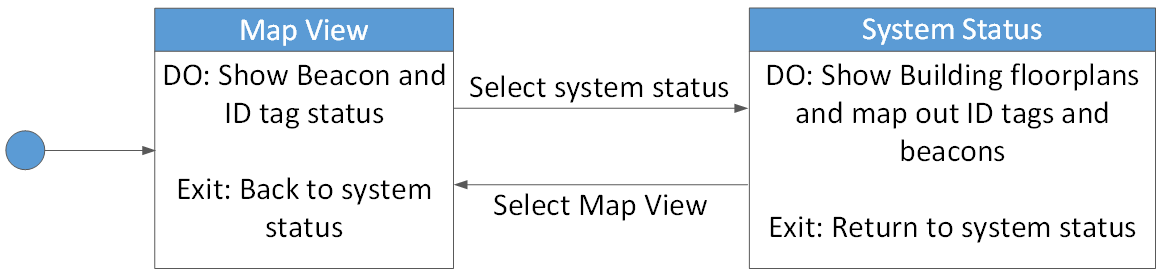
\includegraphics[scale=0.4]{./images/UI_State_FF.png}
    \caption{UI State Diagram - Primary User}
    \label{UISD-1}
\end{figure}
\medskip

The secondary user will be the administrator of the system. For secondary users the interaction is much more complex and require a more in depth level of user interaction. The secondary user interaction state diagram is shown below.

\medskip
\begin{figure}[H]
\centering
    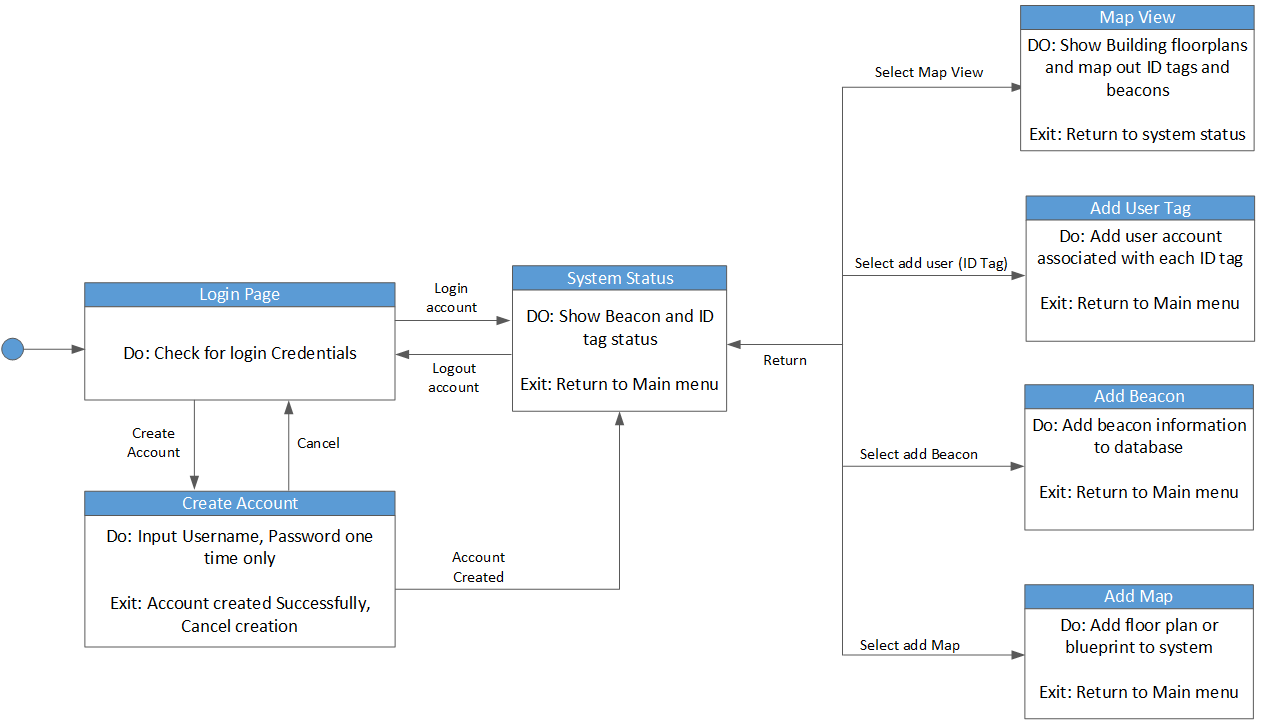
\includegraphics[scale=0.5]{./images/UI_State_IT.png}
    \caption{UI State Diagram - Secondary User}
    \label{UISD-2}
\end{figure}
\medskip



\pagebreak
\subsubsection{UI Mock-Ups}
\medskip
In the Proof of concept a simple console output displaying only the basic information such as the MAC address, RSSI and distance calculations between each beacon and id tag would be shown. Similar to the figure presented below. This UI is just to demonstrate the feasibility of the initial beacon systems.

\medskip
\begin{figure}[H]
\centering
    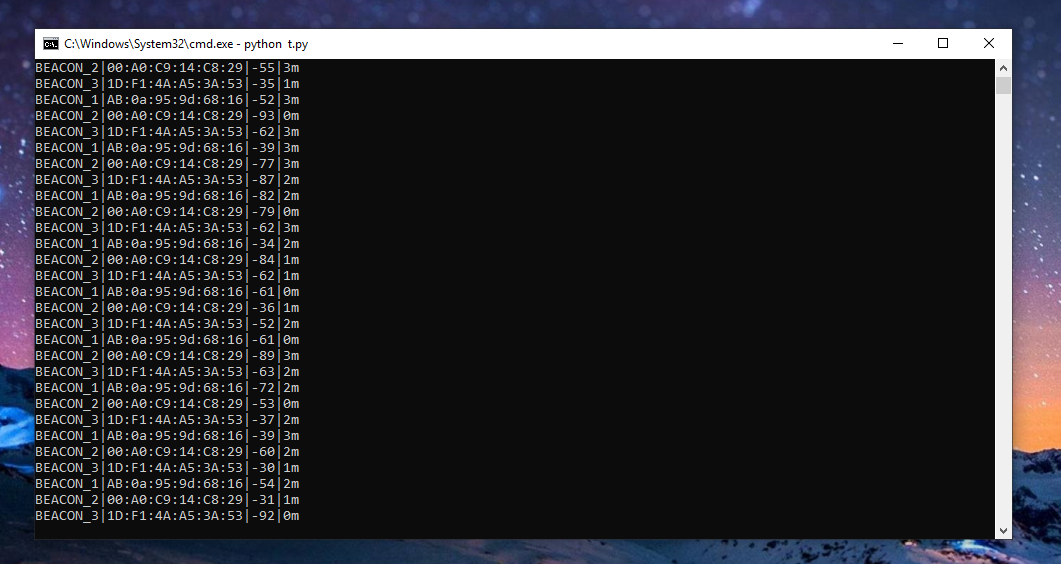
\includegraphics[scale=0.5]{./images/UI_PoC.png}
    \caption{PoC Console UI}
    \label{UI_PoC}
\end{figure}
\medskip

In the prototype phase of development, the user interface would resemble a wireframe of the final implementation. A simple box map is used to display user location in near real time similar to the figure below.

\medskip
\begin{figure}[H]
\centering
    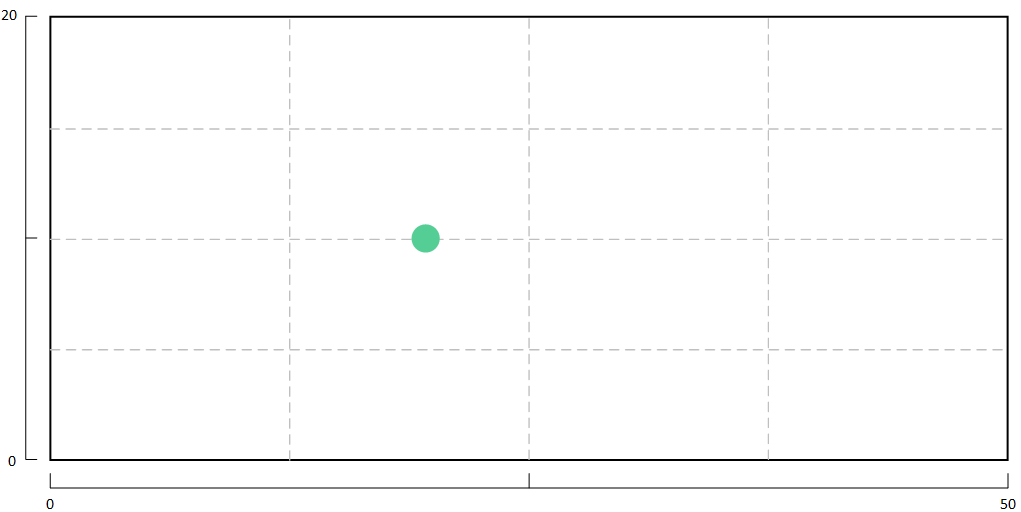
\includegraphics[scale=0.6]{./images/UI_box.png}
    \caption{Prototype Box Map Layout View}
    \label{UI_box}
\end{figure}

\pagebreak

In the Final phase of development the user interface would be complete, resulting in a UI that would fulfil the necessary needs of all users of the system. The primary user would have access to the map view and the system status view shown in figure \ref{map_ff} and \ref{ss_ff}.

\medskip
\begin{figure}[H]
\centering
    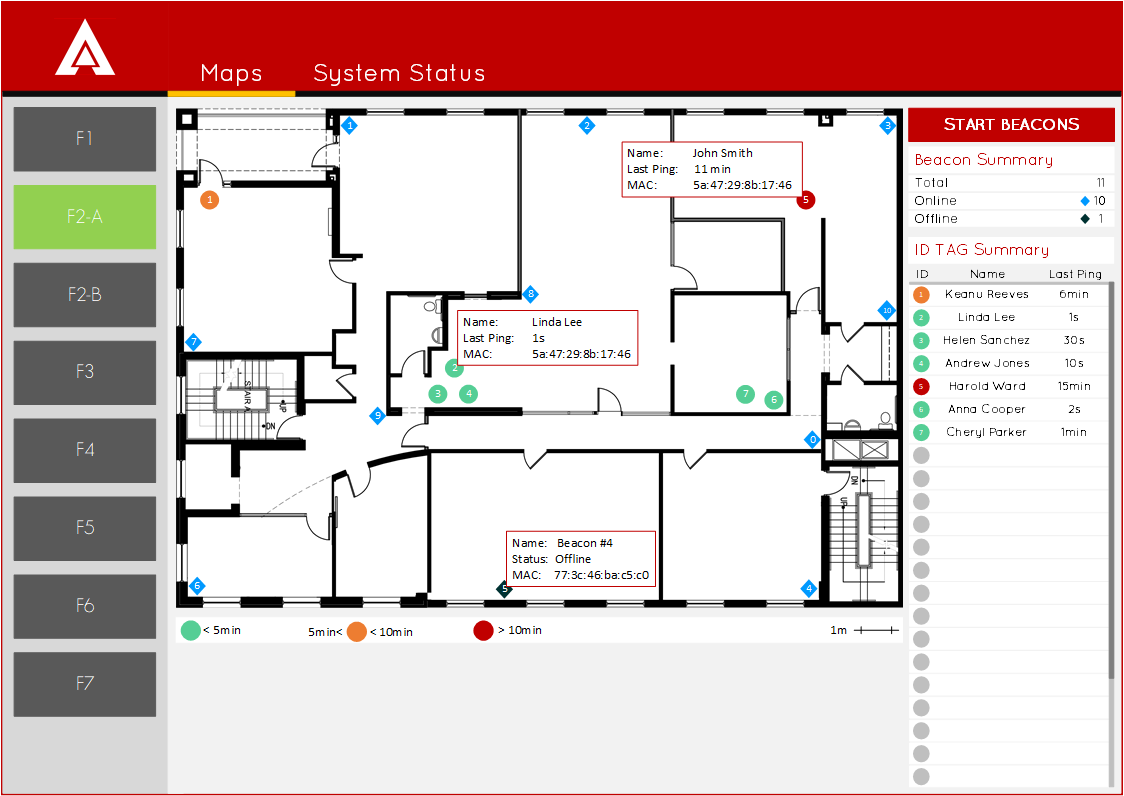
\includegraphics[scale=0.45]{./images/UIMU_map_ff.png}
    \caption{Primary User Map View}
    \label{map_ff}
\end{figure}

\begin{figure}[H]
\centering
    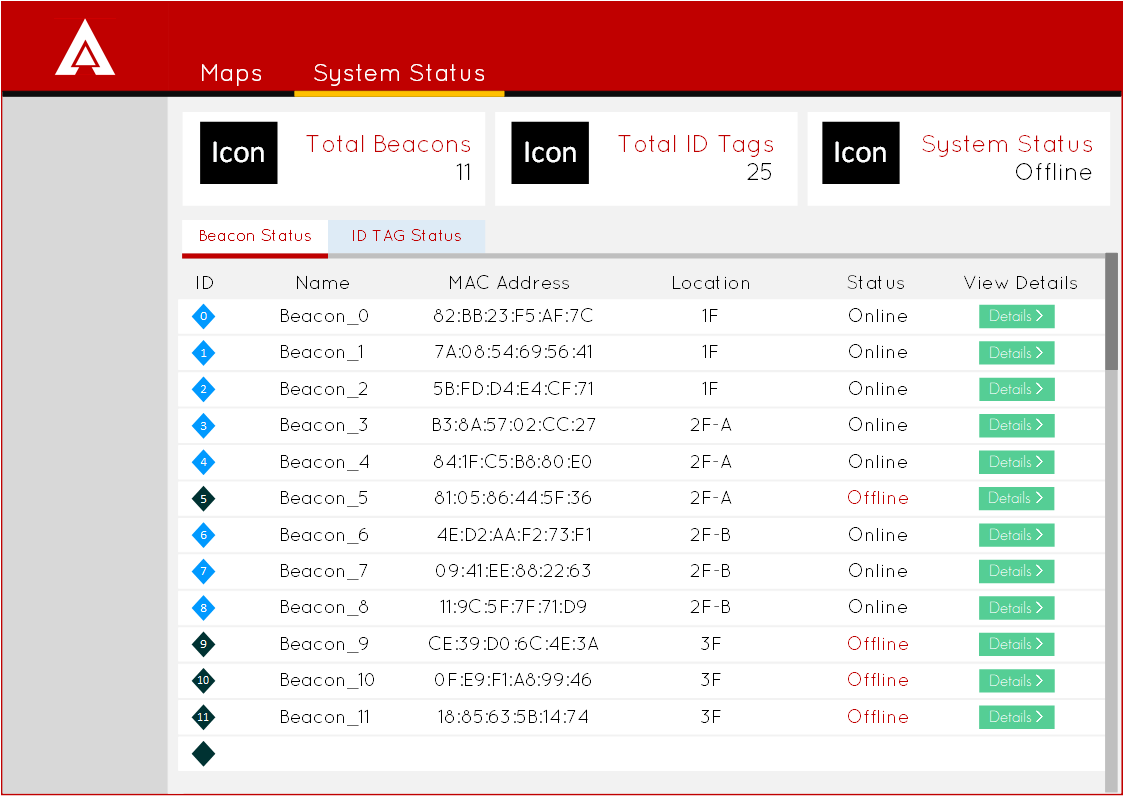
\includegraphics[scale=0.45]{./images/UIMU_status_ff.png}
    \caption{Primary User system status View}
    \label{ss_ff}
\end{figure}
\medskip

\pagebreak
The secondary user, the system administrator will be interacting with the system configurations. The administrator will be performing tasks such as adding/edit beacons, users, and maps or floor plans. The GUI for secondary users are shown in the below figures.

\medskip
\begin{figure}[H]
\centering
    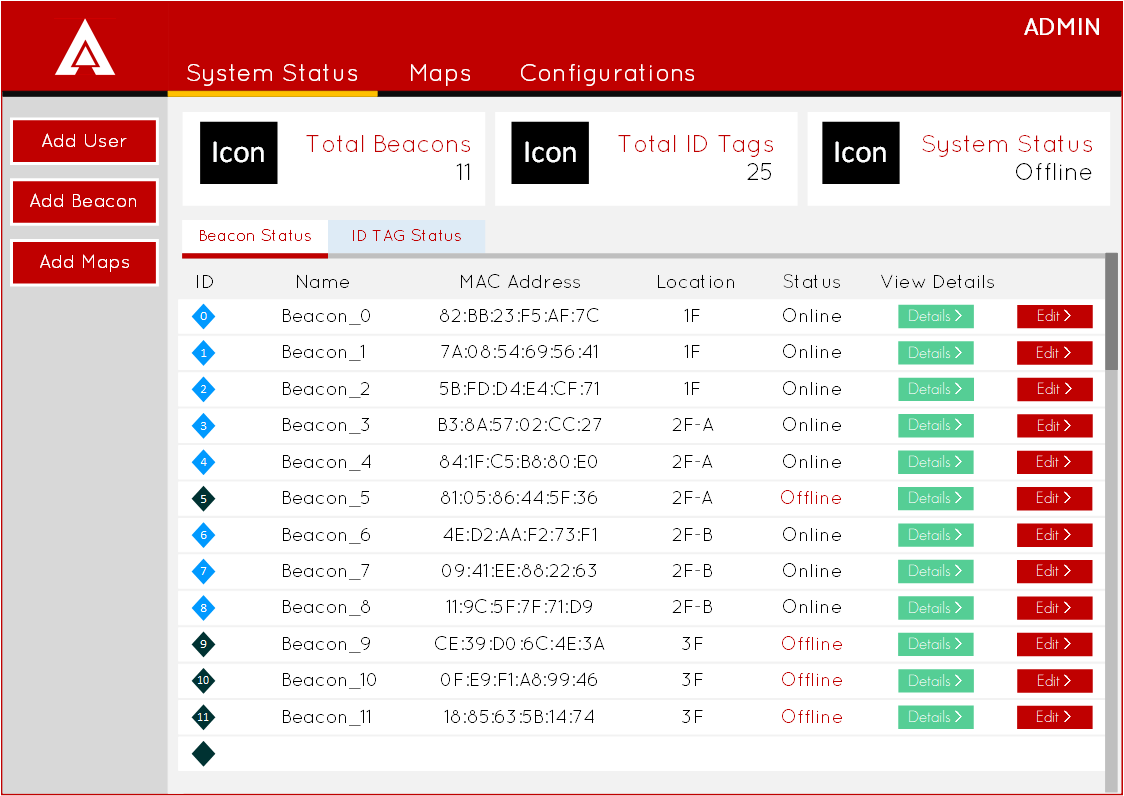
\includegraphics[scale=0.45]{./images/UIMU_status_IT.png}
    \caption{Secondary User System Status View}
    \label{ss_it}
\end{figure}

\medskip
\begin{figure}[H]
\centering
    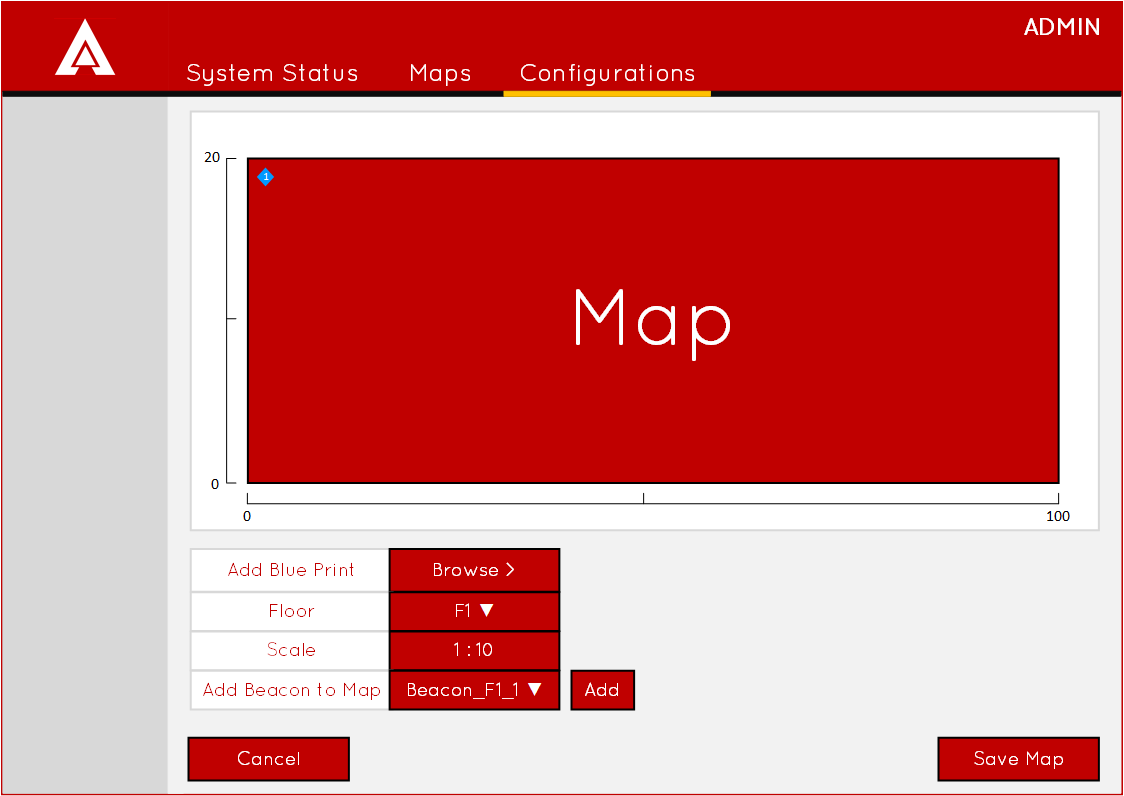
\includegraphics[scale=0.45]{./images/UIMU_add_map.png}
    \caption{Add Map View}
    \label{add_map}
\end{figure}
\pagebreak


\medskip
\begin{figure}[H]
\centering
    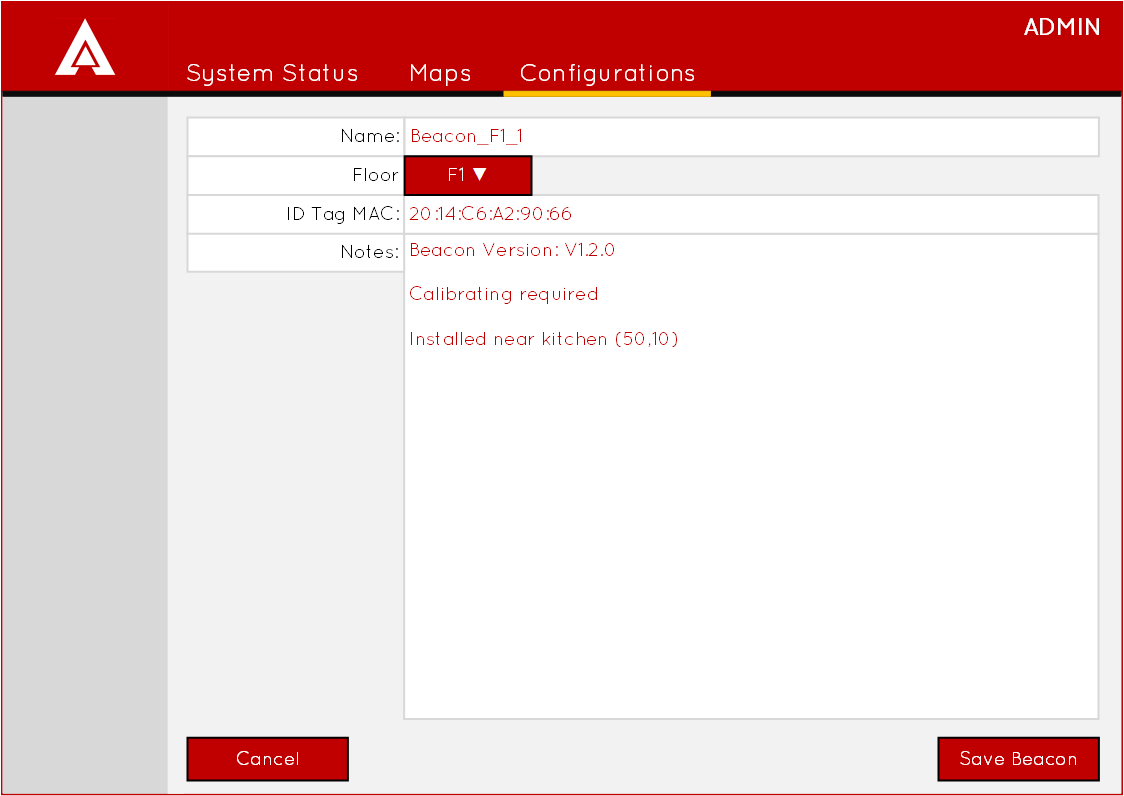
\includegraphics[scale=0.45]{./images/UIMU_add_beacon.png}
    \caption{Add Beacon View}
    \label{add_b}
\end{figure}

\medskip
\begin{figure}[H]
\centering
    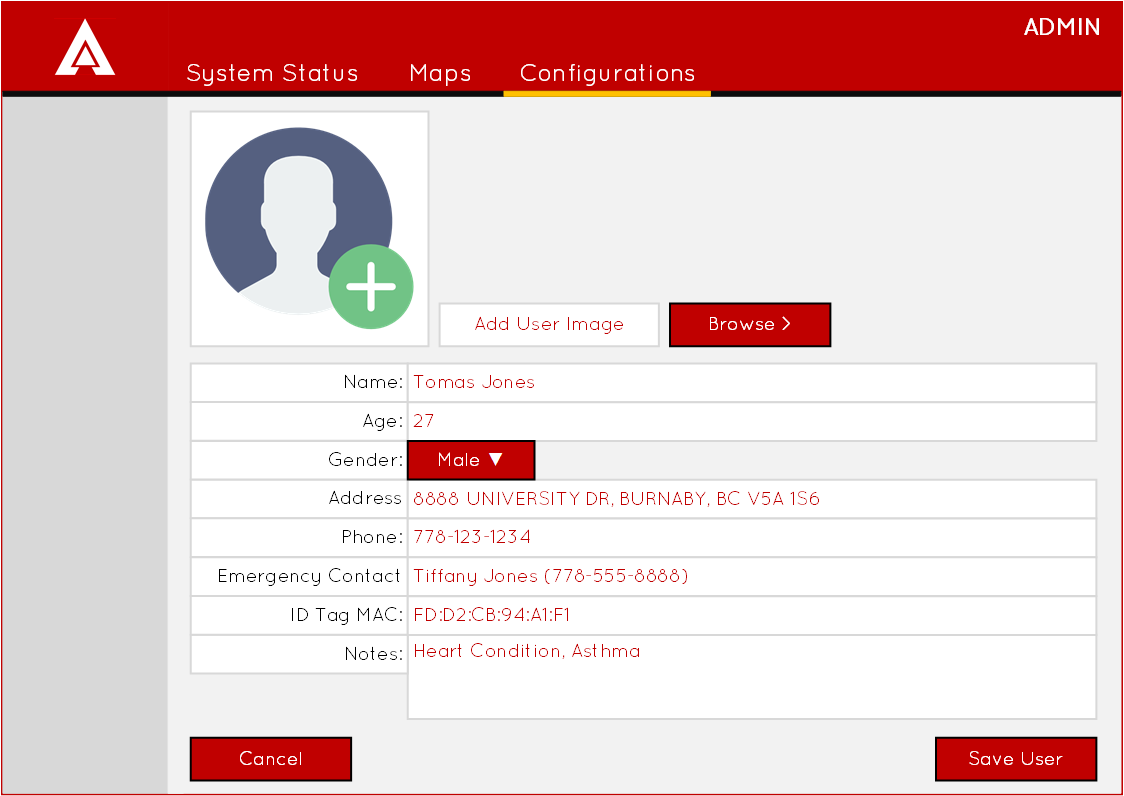
\includegraphics[scale=0.45]{./images/UIMU_add_user.png}
    \caption{Add User View}
    \label{add_user}
\end{figure}






\pagebreak


\subsection{Engineering Standards}
\bigskip
To create an intuitive user interface for optimal user experience, the team at TRIWAVE SYSTEMS will be following several Engineering Standards throughout the development of for the Akriveia Beacon system user interface. The proposed user interface features two branch of components, hardware and software. The hardware components comprising of electronic components such as UWB radio modules and micro-controllers for the device. The software components is split up between data collection from the hardware and data processing. The software also serves as a point of communication and control for the user. The two branches should always inform the user of system operations with easy to understand and highly visible status displayed through the user interface. Interface should also designed in a way that potential errors are kept to a minimum.

\bigskip
These engineering standards published by the \Gls{IEEE}, the \Gls{IEC}, the \Gls{ISO}, and the \Gls{CSA} Group will ensure an intuitive, safe and reliable user interface. Note that some of the standards pertain to the user interface while others pertain to general safety guidelines. The Akriveia Beacon UI design will be built by and tested against the engineering standards listed in the following table.
\bigskip

\def\arraystretch{1.5}
\begin{table}[H]
\centering
\begin{tabular}{ | p{3.5cm} | p{11.5cm}| } 
\hline
\rowcolor{lightgray} \multicolumn{1}{|r|}{\textbf{Standard Code}} & \textbf{Description}\\ 
\hline
\multicolumn{1}{|r|}{CSA-C22.2 NO.61508-1:17} & Functional safety of electrical/electronic/programmableelectronic safety-related systems - Part 1: General requirements \cite{R10-5-1}\\ 
\hline
\multicolumn{1}{|r|}{IEEE 1621-2004} & User Interface Elements in Power Control of Electronic Devices Employed in Office/Consumer Environments \cite{R10-5-2}\\ 
\hline
\multicolumn{1}{|r|}{IEC TR 61997} & Guidelines for the user interface and accompanying word choices \cite{R10-5-3} \\ 
\hline
\multicolumn{1}{|r|}{ISO 20282} & Ease of operation for everyday products \cite{R10-5-4} \\ 
\hline
\multicolumn{1}{|r|}{IEC TR 61997} & Guidelines for the User Interface in Multimedia Equipment for General Purpose Use \cite{R10-5-5} \\ 
\hline
\multicolumn{1}{|r|}{IEEE P360} & Standard for wearable consumer electronic devices \cite{R10-5-6}\\ 
\hline
\multicolumn{1}{|r|}{C22.2 NO.0.23-15} & General Requirements for Battery-Powered Appliances \cite{R10-5-7}\\ 
\hline
\multicolumn{1}{|r|}{IEC 60417} & Graphical symbols for use on equipment \cite{R10-5-8}\\ 
\hline
\multicolumn{1}{|r|}{IEC 62366-1} & Guidance on Usability engineering for software \cite{R10-5-9}\\ 
\hline
\multicolumn{1}{|r|}{ISO/IEC 26907:2009} & Information technology -- Telecommunications and information exchange between systems -- High-rate ultra-wideband PHY and MAC standard \cite{R10-5-10} \\
\hline
\multicolumn{1}{|r|}{ISO/IEC 24730-62:2013} & Information technology -- Real time locating systems (RTLS) -- Part 62: High rate pulse repetition frequency Ultra Wide Band (UWB) air interface \cite{R10-5-11}\\ 
\hline
\end{tabular}
\caption{Engineering Standards}
\end{table}	










\pagebreak


\subsection{Analytical Usability Testing}
\bigskip
The Akriveia beacon user interface will be tested to determine the state of its usability at various stages of development. The analytical testing phase outlines testing procedure that will be done by the engineering and design team using heuristic usability evaluations. Each evaluator will independently examine the UI and check for compliance and usability. After collecting the results the team will discuss and compile possible solutions to usability issues and generate a list of solutions. Finally, the redesign will be implemented and regression testing will be done. The analytical usability testing will take place during the prototype and final product phases of development as the user interface is well defined during these two stages. The testing procedure will follow the steps described below.

\bigskip



\textbf{Step 1:} Usability Research Data Collection\\
\medskip
The first step is to collect the data generated by the usability test. Each evaluator will perform simple tasks outlined in the testing appendix (section \#). From the procedures performed issues will be highlighted and documented. Each issue will have the following:
\begin{itemize}
\setlength\itemsep{0.1mm}
	\item An issue identification (ID).
	\item Note where it happened (screen, module, UI widget, flow, etc.).
	\item Task the user was engaging in.
	\item Concise description of the issue.
\end{itemize}
Data collected will be shown in a table similar to the table below:

\def\arraystretch{1.5}
\begin{table}[H]
\centering
\begin{tabular}{ | p{0.5cm} | p{2cm}| p{5cm} | p{5cm} | p{0.5cm} | p{0.5cm} | p{0.5cm}|} 
\hline 
ID & Where & Task & Description & P1 & P2 & P3 \\
\hline
1 & Login Page & Login with wrong Password & No error message for wrong user name input & X & - & - \\
\hline
2 & Map View & Click on beacon icon & Beacon info text too small & - & X & X \\
\hline
\end{tabular}
\caption{Usability test results}
\end{table}	



\textbf{Step 2:} Issue prioritization\\
\medskip
Once sufficient testing has been performed by evaluators of the team, issues must be prioritized as time and resources are limited for this project. Each usability issue receives a grade of severity, influenced by factors such as:
\begin{itemize}
\setlength\itemsep{0.1mm}
	\item Task criticality: Impact on user if the task is not accomplished.
	\item Issue frequency: How many times an issue has occurred with various participants.
	\item Issue impact: How much has it impacted the user trying to accomplish the task.
\end{itemize}

\bigskip



\textbf{Step 3:} Solution Generation\\
\medskip
With the combined feedback and evaluations, the engineers at TRIWAVE SYSTEMS will re-evaluate possible UI designs for each usability issue that occurred during testing to determine the best and optional solution. A list of recommendations and solutions will be generated with usability test results. For each design decision several alternative solutions must be generated to include other possible ways to address the issue. 








\pagebreak


\subsection{Empirical Usability Testing}
\medskip
This section details the completed empirical usability testing with users and outlines the methods of testing required for future implementations. Empirical usability testing will be carried out by the engineers at TRIWAVE SYSTEMS to systematically determine the usability of the user interface design of the Akriveia Beacon System. 

\bigskip
During empirical usability testing, testing will be carried out in cycles with real users consists of volunteer participants. The first cycle occurs near the end of the Prototype phase and the second cycle occurs near the end of the Final Product phase. Testing will be done with two small groups of participants that are unfamiliar with project development environment. First group will be asked to perform usability test cases outlined in Appendix A. An observer will document actions and observations of the testing process as well as to keep note of average time to complete each task, the amount of errors and error rate, number of tasks completed, and perform a sequence analysis. Issues will be represented similar to the method mentions in 10.6 Analytical usability testing. With the collected data the designers will re-evaluate the user interface for possible solutions for issues. After re-design and implementation a second small group of participants will be asked to perform the same tasks as the first group

\bigskip
From the results generated by participants the following usability elements will be addressed throughout the two testing cycles and development stages. 

\medskip
\begin{itemize}
\setlength\itemsep{0.1mm}
	\item \textbf{Easability:} The familiarity and intuitiveness of the system and how comfortable the users are with the user interfaces in general. 
	\item \textbf{Navigation:} The reliability of the navigation sequences are, how easy is it for the users to understand paths, and/or short cuts. Can the users easily retrace their steps or go back to previous states if they have made a mistake?
	\item \textbf{Responsiveness:} Does the users receive sufficient feedback from interacting with the system? 
	\item \textbf{Intuitiveness:} How quickly can a new user familiarize themselves with the user interface? Whether or not the users are able to perform tasks within a certain amount of time?
	\item \textbf{Robustness:} Safety and reliability of the device and system are addressed by eliminating or minimizing potential error (slips and mistakes) and enabling error recovery.
\end{itemize}

\medskip
By following these usability testing methods mentioned above for the Akriveia Beacon, the engineers and designers at TRIWAVES SYSTEMS can ensure a reliable and intuitive user interface will be produced to meet the needs of its end users. 

\pagebreak


\subsection{Conclusion}
\medskip
The User Interface design for the proof-of-concept, prototype, and the final product of the Akrieva Beacon system developed by TRIWAVE SYSTEMS is detailed in this appendix section. Currently the conceptual framework of the Akriveia Beacon system is under development, with the primary circuitry and initial interfaces under design and early implementations. The major feature to be implemented is the wireless communication interfaces and protocols between anchor beacons and ID tags; the control and data processing unit are also in parallel development. The final project goal is to showcase the Akriveia as an accurate, reliable, modular, and simple solution in providing automated indoor location tracking with near real time and multi-tracking capabilities.  

\bigskip
This appendix outlines a study of the user analysis, and technical analysis for interaction between the system and its intended users. As well as an overview of engineering safety and standards to ensure that the Akriveia Beacon system is safe and reliable for its designated users. Analytical usability testing and empirical usability testing will be performed to ensure that the basic system functionality, aesthetics, stability, and reliability are completely sufficient with of all planned requirements satisfied. 

\bigskip
With the help of the Akriveia Beacon system, under the intended scenario, primary users of the system such as fire fighters and first responders will be able to locate trapped personnel with minimized search time; therefore, lowering rescue time and allowing for higher survival rate for trapped victims during the event of disasters. 














\pagebreak
\printbibliography[heading=bibnumbered, title={Appendix References},type=book]
\pagebreak


%\end{document}



\end{document}
